\part{Statistical and Learning Systems}

\section{Statistical Learning}

\subsection{Statistical Inference Foundations}
% Models, estimators, bias/variance, likelihood, Bayesian/frequentist viewpoints.

\subsection{Risk Minimization}
% Loss functions, empirical risk, expected risk, consistency, bias-variance tradeoff.

\subsection{Linear and Generalized Linear Models}
% Regression, classification, logistic regression, GLMs, regularization.

\subsection{Regularization and Model Selection}
% Ridge, lasso, sparsity, cross-validation, information criteria.

\subsection{Kernels and Nonlinear Methods}
% RKHS intuition, kernel ridge regression, SVMs, Gaussian processes as learning models.

\subsection{Trees, Ensembles, and Boosting}
% Decision trees, bagging, random forests, boosting, gradient boosting.

\subsection{Generalization Theory}
% VC dimension, Rademacher complexity preview, concentration, stability.

% Sources: Hastie-Tibshirani-Friedman, The Elements of Statistical Learning; Bishop, Pattern Recognition and Machine Learning; Murphy selectively.

\section{Deep Learning and Representation Systems}

\subsection{Neural Network Foundations}
% Feedforward networks, activation functions, backpropagation, universal approximation.

\subsubsection{Deep Feedforward Networks}

\begin{remark} \hlt{Deep Feedforward Networks (DFNs)}\\
Defines a mapping $\bm{y} = f(\bm{x}; \bm{\theta})$ and learns value of parameters $\bm{\theta}$ that results in best function approximation.
\end{remark}

\begin{remark} \hlt{Linear Models}\\
Linear models may fit data efficiently and reliably, either in closed form or with convex optimisation.\\
Model capacity limited to linear functions, does not model interaction between any two input variables
\end{remark}

\begin{remark} \hlt{Nonlinear Models}\\
To represent nonlinear functions of $\bm{x}$, apply linear model to transformed input $\phi(\bm{x})$ where $\phi$ is a nonlinear transformation. Kernel trick may be applied to obtain nonlinear learning algorithm. To choose mapping $\phi$:
\begin{enumerate}[label=\roman*.]
\setlength{\itemsep}{0pt}
\item Choose generic $\phi$, such as that used by kernel machines based on RBF kernel.\\
If $\phi(\bm{x})$ is of high enough dimension, can find enough capacity to fit training set, but generalisations to test set remains poor. Mappings are based on principle of local smoothness and do not encode enough prior information to solve advanced problems.
\item Manually engineer $\phi$. Requires decades of human effort for each task, and practitioners specialising in different domains (i.e, speech recognition, computer vision) with little transfer between domains.
\item Learn $\phi$ through deep learning. Model is $y = f(\bm{x}; \bm{\theta}, \bm{w}) = \phi(\bm{x}; \bm{\theta})^T \bm{w}$, where parameters $\bm{\theta}$ can be used to learn $\phi$ from broad class of functions, and parameters $\bm{w}$ that map from $\phi(\bm{x})$ to desired output.\\
Do not require training problem to be convex, and only require finding the right general function.
\end{enumerate}
\end{remark}

\begin{definition} \hlt{Cost Functions}
\begin{enumerate}[label=\roman*.]
\setlength{\itemsep}{0pt}
\item Learning Conditional Distributions with Maximum Likelihood: cost function is negative log-likelihood, which is the cross-entropy between training data and model distribution:
\begin{equation*}
J(\bm{\theta}) = - \mathbb{E}_{\bm{x}, \bm{y} \sim \hat{p}_{\text{data}}} \log p_{\text{model}}(\bm{y} \ \vert \ \bm{x}) \nonumber
\end{equation*}
Specific form of cost function changes from model to model, depending on form of $\log p_{\text{model}}$.\\
Method removes the burden of designing cost functions for each model, as specifying a model $p(\bm{y} \ \vert \ \bm{x})$ automatically determines a cost function $\log p(\bm{y} \ \vert \ \bm{x})$.\\
Gradient of cost function for neural networks must be large and predictable enough to serve as good guide for the learning algorithm. The negative log-likelihood helps to avoid saturation of the function.
\item Learning Conditional Statistics: to learn just one conditional statistic of $\bm{y}$ given $\bm{x}$.\\
With sufficiently powerful neural network, this can represent any function $f$ from a wide class of function, limited by features of continuity and boundedness. Hence the cost function is a functional. Learning is choosing a functional rather than a set of parameters.\\
By calculus of variation	, solving the optimisation problem yields the below function,
\begin{align*}
f^* &= \arg \min_f \mathbb{E}_{\bm{x}, \bm{y} \sim p_{\text{data}}} \Vert \bm{y} - f(\bm{x}) \Vert^2 \nonumber \\
f^* &= \mathbb{E}_{\bm{y} \sim p_{\text{data}}(\bm{y} \ \vert \ \bm{x})} [\bm{y}] \nonumber
\end{align*}
If infinitely many samples from the true data-generating distribution could be trained, then minimising the mean squared error cost function gives a function that predicts mean of $\bm{y}$ for each value of $\bm{x}$.\\
A second result from calculus of variations is:
\begin{align*}
f^* = \arg \min_f \mathbb{E}_{\bm{x}, \bm{y} \sim p_{\text{data}}} \Vert \bm{y} - f(\bm{x}) \Vert_1 \nonumber
\end{align*}
which is a function that predicts the median value of $\bm{y}$ for each $\bm{x}$. This is the mean absolute error.\\
Note that mean squared error and mean absolute error often lead to poor results when used with gradient-based optimisation. Output units that saturate may produce very small gradients when combined with these cost functions. Hence the reason that cross-entropy cost function is more popular.
\end{enumerate}
\end{definition}

\begin{definition} \hlt{Output Units}
\begin{enumerate}[label=\roman*.]
\setlength{\itemsep}{0pt}
\item Linear Units: base on affine transformation with no nonlinearity.\\
Given features $\bm{h}$, a layer of output units produces vector $\hat{\bm{y}} = \bm{W}^T \bm{h} + \bm{b}$. Linear output layers are used to produce mean of conditional Gaussian distribution:
\begin{equation*}
p(\bm{y} \ \vert \ \bm{x}) = \mathcal{N}(\bm{y}; \hat{\bm{y}}, \bm{I}) \nonumber
\end{equation*}
Maximising log-likelihood is equivalent to minimising mean squared error.\\
Linear units do not saturate, hence may be used for wide variety of optimisation algorithms.
\item Sigmoid Units: define Bernoulli distribution $y$ conditioned on $\bm{x}$. Neural net to predict $P(y = 1 \ \vert \ \bm{x})$, which lies in interval $[0,1]$. The sigmoid unit is defined by
\begin{equation*}
\hat{y} = \sigma(\bm{w}^T \bm{h} + b) \nonumber
\end{equation*}
where $\sigma$ is the logistic sigmoid function.\\
Note that the cost function used with maximum likelihood is $- \log P(y \ \vert \ \bm{x})$, preventing saturation.\\
The loss function for MLE of Bernoulli parametrised by sigmoid is
\begin{equation*}
J(\bm{\theta}) = - \log P(y \ \vert \ \bm{x}) = - \log \sigma((2y - 1)z) = \zeta((1-2y)z) \nonumber
\end{equation*}
Function saturates only when $(1-2y)z$ is very negative, i.e., when model has the right answer.
\item Softmax Units: used to represent probability distribution over $n$ different classes.\\
A linear layer predicts unnormalised log probabilities:
\begin{equation*}
\bm{z} = \bm{W}^T \bm{h} + \bm{b} \nonumber
\end{equation*}
where $z_i = \log \tilde{P}(y=i \ \vert \ \bm{x})$. Softmax function is then
\begin{equation*}
\text{softmax}(\bm{z})_i = \frac{\exp(z_i)}{\sum_j \exp(z_j)} \nonumber
\end{equation*}
The function is to maximise $\log P(y=i ; \bm{z}) = \log \text{softmax}(\bm{z})_i = z_i - \log \sum_{j} \exp(z_j)$.\\
Note that the input $z_i$ always has direct contribution to cost function, and the term cannot saturate.\\
Un-regularised maximum likelihood will drive the model to learn parameters that drive the softmax to predict fraction of counts for each outcome observed in the training set:
\begin{equation*}
\text{softmax}(z(\bm{x}; \bm{\theta}))_i \approx \frac{\sum\limits_{j=1}^{m} \bm{1}_{y^{(j)}=i, \bm{x}^{(j)} = x}}{\sum\limits_{j=1}^m \bm{1}_{\bm{x}^{(j)}=x}} \nonumber
\end{equation*}
Note that objective functions other than log-likelihood does not work well with softmax function. Squared error is poor loss function for softmax units, and can fail to train the model to change its output.\\
Softmax function can saturate, and many functions based on softmax also saturate, unless they are able to invert the saturating activating function.
\item Other Output Types: generally, given a conditional distribution $p(\bm{y} \ \vert \ \bm{x}; \ \bm{\theta})$, principle of maximum likelihood suggests using $- \log p(\bm{y} \ \vert \ \bm{x}; \ \bm{\theta})$ as the cost function.\\
Neural networks represent a function $f(\bm{x}; \bm{\theta}) = \bm{\omega}$. The outputs of the function are not direct predictions of value $\bm{y}$, but the parameters for distribution over $\bm{y}$. The loss function is then $- \log p(\bm{y} ; \bm{\omega}(\bm{x}))$.
\end{enumerate}
\end{definition}

\begin{remark} \hlt{Learning Distribution Parameters}
\begin{enumerate}[label=\roman*.]
\setlength{\itemsep}{0pt}
\item Heteroscedastic Model: to predict different variance in $\bm{y}$ for different values of $\bm{x}$, formulate the Gaussian distribution using precision rather than variance. In multi-variate case, the diagonal precision matrix is used, $\text{diag}(\bm{\beta})$. The log-likelihood of Gaussian distribution parametrised by $\bm{\beta}$ involves only multiplication by $\beta_i$ and addition of $\log \bm{\beta}_i$. The gradient of these operations are well-behaved.\\
Let $\bm{\alpha}$ be raw activation of the model used to determine diagonal precision. The softplus function may be used to obtain a positive precision vector $\bm{\beta} = \zeta(\bm{\alpha})$. Same strategy applies equally if using variance variance or standard deviation rather than precision.\\
If covariance is full and conditional, then parametrisation must be chosen that guarantees positive-definiteness of predicted covariance matrix.
\begin{equation*}
\bm{\Sigma}(\bm{x}) = \bm{B}(\bm{x}) \bm{B}^T(\bm{x}) \nonumber
\end{equation*}
where $\bm{B}$ is unconstrained square matrix. Note that if matrix is full rank, then computing likelihood requires $O(d^3)$ a $d \times d$ matrix for the determinant and inverse of $\bm{\Sigma}(\bm{x})$.
\item Mixture Density Networks: to perform multimodal regression (predict real values that come from conditional distribution $p(\bm{y} \ \vert \ \bm{x})$) that can have several different peaks in $\bm{y}$ for the same $\bm{x}$.
\begin{equation*}
p(\bm{y} \ \vert \ \bm{x}) = \sum\limits_{i=1}^n p(c=i \ \vert \ \bm{x}) \mathcal{N}(\bm{y}; \bm{\mu}^{(i)} (\bm{x}), \bm{\Sigma}^{(i)} (\bm{x})) \nonumber
\end{equation*}
The neural network will have three outputs:
\begin{enumerate}[label=\arabic*.]
\setlength{\itemsep}{0pt}
\item Mixture components $p(c = i \ \vert \ \bm{x})$, forming a multinoulli distribution over $n$ different components with latent variable $c$, obtained by softmax over $n$-dimensional vector.
\item Means $\bm{\mu}^{(i)}(\bm{x})$
\item Covariances $\bm{\Sigma}^{(i)}(\bm{x})$
\end{enumerate}
Gradient-based optimisation of conditional Gaussian mixtures can be unreliable as the divisions can be numerically unstable. May be solved by clipping gradients, or scaling gradients heuristically.
\end{enumerate}
\end{remark}

\begin{definition} \hlt{Hidden Units}\\
Even if hidden units are not differentiable at all input points, gradient descent still performs well enough as the training algorithms do not usually arrive at local minimum of cost function, but reduce its value significantly.\\
Most hidden units has input vector $\bm{x}$, computes an affine transformation $\bm{z} = \bm{W}^T \bm{x} + \bm{b}$, then applying element-wise non-linear function $g(\bm{z})$.
\begin{enumerate}[label=\roman*.]
\setlength{\itemsep}{0pt}
\item Rectified Linear Units (ReLUs): uses activation function $g(z) = \max \{0, z\}$.\\
Typically used on top of an affine transformation $\bm{h} = g(\bm{W}^T \bm{x} + \bm{b})$. In initialisation, set all elements of $\bm{b}$ to small positive values, so that ReLUs will be initially active for most inputs in training set.\\
Generalisations of ReLUs have non-zero slope $\alpha_i$ for $z_i < 0$: $h_i = \max(0, z_i) + \alpha_i \min(0, z_i)$.
\begin{enumerate}[label=\arabic*.]
\setlength{\itemsep}{0pt}
\item Absolute Value Rectification: sets $\alpha_i = -1$ to obtain $g(z) = \abs{z}$. Used for object recognition from images, to seek features that are invariant under polarity reversal of input illumination.
\item Leaky ReLU: fixes $\alpha_i$ to small positive value
\item Parametric ReU: treats $\alpha_i$ as a learnable parameter
\end{enumerate}
\item Maxout Units: divide $\bm{z}$ into groups of $k$ values. Each maxout unit then outputs maximum element of one of these groups: $g(\bm{z})_i = \max_{j \in \mathbb{G}^{(i)}} z_j$, where $\mathbb{G}^{(i)}$ is indices of inputs for group $i$, which is $\{(i-1)k + 1, \ldots, ik\}$.\\
This allows learning of piecewise linear function that responds to multiple directions in input $\bm{x}$ space .\\
Maxout units learn the activation function itself. With large $k$, maxout unit can learn to approximate any convex function. Each maxout unit is parametrised by $k$ weight vectors, hence need more regularisation than ReLUs. Benefits include:
\begin{enumerate}[label=\arabic*.]
\setlength{\itemsep}{0pt}
\item Can work well without regularisation if training set is large and number of pieces per unit is low.
\item Can gain statistical and computation advantages by requiring fewer parameters.
\item Have redundancy that resists catastrophic forgetting, where neural networks forgot how to perform tasks that were trained on in the past.
\end{enumerate}
\item Logistic Sigmoid and Hyperbolic Tangent: the logistic sigmoid activation function is $g(z) = \sigma(z)$, and the hyperbolic tangent activation function is $g(z) = \tanh(z)$. Note that $\tanh(z) = 2 \sigma(2z) - 1$.\\
Sigmoidal units saturate across most of the domain, which makes gradient-based learning very difficult. Hence the use in hidden units in feedforward networks is now discouraged.\\
If sigmoidal activation function must be used, hyperbolic tangent activation function performs better, as it resembles identity function more closely. Training $\hat{y} = \bm{w}^T \tanh(\bm{U}^T \tanh(\bm{V}^T \bm{x}))$ resembles training a linear model $\hat{y} = \bm{w}^T \bm{U}^T \bm{V}^T \bm{x}$ as long as the activations of the network can be kept small.\\
Sigmoidal functions are more common in recurrent networks, probabilities models, auto-encoders
\item Linear Unit: consider neural network layer with $n$ inputs, $p$ outputs, $\bm{h} = g(\bm{W}^T \bm{x} + \bm{b})$. Replace with two layers, one using weight matrix $\bm{U}$ and the other using weight matrix $\bm{V}$. If first layer has no activation function, then the factored approach is to compute $\bm{h} = g(\bm{V}^T \bm{U}^T \bm{x} + \bm{b})$. If $\bm{U}$ produces $q$ outputs, then $\bm{U}$ and $\bm{V}$ together only contains $(n+p)q$ parameters, while $\bm{W}$ contains $np$ parameters. For small $q$, this is considerable saving in parameters, while the cost is constraining linear transformation to be low rank. This is an efficient way of reducing number of parameters in the model.
\item Softmax: naturally represent probability distribution over discrete variable with $k$ possible values. Used only in more advanced architectures that explicitly learn to manipulate memory.
\item Radial Basis Function (RBF): function becomes more active as $\bm{x}$ approaches a template $\bm{W}_{:, i}$. As it saturates to $0$ for most $\bm{x}$, it can be difficult to optimise.
\begin{equation*}
h_t = \exp \left( - \frac{1}{\sigma^2_i} \Vert \bm{W}_{:, i} - \bm{x} \Vert^2 \right) \nonumber
\end{equation*}
\item Softplus: smooth version of rectifier for functional approximation and for conditional distributions of undirected probabilistic models. Usage is generally discouraged.
\begin{equation*}
g(a) = \zeta(a) = \log(1 + e^a) \nonumber
\end{equation*}
\item Hard $\tanh$: shaped similarly to $\tanh$ but bounded.
\begin{equation*}
g(a) = \max(-1, \min(1,a)) \nonumber
\end{equation*}
\end{enumerate}
\end{definition}

\begin{theorem} \hlt{Universal Approximation Theorem}\\
A feedforward network with linear output layer and at least one hidden layer with any 'squashing' activation function can approximate any Borel measurable function from one finite-dimensional space to another with any desired non-zero amount of error, provided the network is given enough hidden units.
\end{theorem}

\begin{method} \hlt{Architecture Design}\\
Neural network layers are arranged in a chain structure, with each layer being a function of preceding layer.
\begin{align}
\bm{h}^{(1)} &= g^{(1)} (\bm{W}^{(1)T} \bm{x} + \bm{b}^{(1)}) \nonumber \\
\bm{h}^{(k)} &= g^{(k)} (\bm{W}^{(k)T} \bm{h}^{(k-1)} + \bm{b}^{(k)}), \ \ \ k \geq 2 \nonumber
\end{align}
The main considerations are the depth of network and width of each layer. Deeper networks use far fewer units per layers and far fewer parameters, and often generalise to the test set, but are harder to optimise.
\end{method}

\begin{remark} \hlt{Depth of Network and Universal Approximation Theorem}\\
A feedforward network with single layer is sufficient to represent any function, but the layer may be infeasibly large and fail to learn and generalise correctly. Using deeper models can reduce number of units required to represent the desired function and can reduce generalisation error.\\
Shallow networks with broad family of non-polynomial activation functions have universal approximation properties. Piecewise linear networks can represent functions with number of regions that is exponential to depth.\\
The number of linear regions carved out by deep rectifier network with $d$ inputs, depth $l$, and $n$ units per hidden layer is $O(\binom{n}{d}^{d(d-1)} n^d)$. For maxout networks with $k$ filters per unit, this is $O(k^{(k-1)+d})$.
\end{remark}

\begin{remark} \hlt{Backpropagation}\\
To calculate the gradient of loss function with respect to each of individual parameters of the neural network.\\
Model training begins with random initialisation of weights and biases.
\begin{enumerate}[label=\roman*.]
\setlength{\itemsep}{0pt}
\item Forward pass: input is sampled from training data. Nodes receive input vector and passes their value (multiplied by random initial weight) to nodes of first hidden layer. The hidden units take weighted sum of these output values as an input to the activation function, whose output is used for next hidden layer.
\item Error computation: the final output of the network is compared to the ground truth, difference is calculated for the error value.
\item Backwards pass: the error value computed earlier is used to compute the gradient of loss function. The gradient is then propagated back through the network, and the weights are updated according to their contribution to the error. The learning rate determines the size of weight updates.
\item Weights update: the weights are updated in opposite direction of the gradient
\end{enumerate}
\end{remark}


\begin{breakablealgorithm}
\caption{Backpropagation Learning Algorithm}
\begin{algorithmic}
\Require \\
A set of training examples $\mathcal{D} = \{(x_i, y_i)\}_{i=1}^n$\\
A multilayer network with $L$ layers, weights $w_{ij}^l$, and activation function $f$\\
Loss function $J(y, o)$\\
Learning rate $0 < \alpha < 1$\\
Number of epochs \textit{epochs}.\\
    
\State \textit{Initialize all weights:} 
\For{$w_{ij}^l$ in the network}
\State $w_{ij}^l \gets \text{small random number}$
\EndFor\\

\For{$i = 1 \text{ to } \textit{epochs}$}
\ForAll{training examples $(x,y) \in \mathcal{D}$}\\
\State \textit{Propagate the inputs forward to compute the outputs}
\ForAll{neurons $i$ in the input layer}
\State $a_i^0 \gets x_i$
\EndFor \\
\For{$l = 2 \text{ to } L$}
\ForAll{neurons $i$ in layer $l$}
\State $z_i^l \gets \displaystyle\sum_j w_{ij}^l\,a_j^{l-1}$
\State $a_i^l \gets f\bigl(z_i^l\bigr)$
\EndFor
\EndFor\\

\State \textit{Propagate deltas backward from output layer to input layer}
\ForAll{neurone $i$ in the output layer}
\State \textit{Let  $o_i \equiv a_i^L$ be output of neurone $i$}
\State $\delta_i^L \gets \dfrac{\partial J(y_i,o_i)}{\partial o_i}\,f'\bigl(z_i^L\bigr)$
\EndFor\\
\For{$l = L-1 \text{ to } 1$}
\ForAll{neurons $i$ in layer $l$}
\State $\delta_i^l \gets f'\bigl(z_i^l\bigr) \sum_j\bigl(w_{ji}^{l+1}\,\delta_j^{l+1}\bigr)$
\EndFor
\EndFor\\

\State \textit{Update weights using the deltas}
\ForAll{$w_{ij}^l$ in the network}
\State $w_{ij}^l \gets w_{ij}^l - \alpha\,\delta_i^l\,a_j^{l-1}$
      \EndFor
    \EndFor
  \EndFor
\end{algorithmic}
\end{breakablealgorithm}

\begin{example} \hlt{Backpropagation Computation Example (Matt \cite{mazur_backpropagation_2015})}
\begin{figure}[H]
\centering
\scalebox{0.75}{\tikzset{
    neuron/.style={circle, draw, minimum size=1cm},
    input neuron/.style={neuron, fill=green!20},
    hidden neuron/.style={neuron, fill=blue!20},
    output neuron/.style={neuron, fill=blue!20},
    bias neuron/.style={neuron, fill=gray!20},
    connection/.style={->,thick},
    biasconnection/.style={->,thick,draw=gray},
    mylabel/.style={midway,fill=none,inner sep=1pt}
}

\begin{tikzpicture}[node distance=1.8cm and 2.5cm, font=\sffamily\small]

% Nodes
\node[input neuron] (i1) {i1};
\node[input neuron, below=of i1] (i2) {i2};

\node[hidden neuron, right=of i1] (h1) {h1};
\node[hidden neuron, below=of h1] (h2) {h2};

\node[output neuron, right=of h1] (o1) {o1};
\node[output neuron, below=of o1] (o2) {o2};

\node[bias neuron, below=of i2] (b1) {1};
\node[bias neuron, below=of h2] (b2) {1};

% Connections
\draw[connection] (i1) -- (h1) node[mylabel,above] {.15 w1};
\draw[connection] (i1) -- (h2) node[mylabel,below right =-1.2cm of i1] {\ .20 w2};
\draw[connection] (i2) -- (h1) node[mylabel,above right =-1.2cm of i2] {\ .25 w3};
\draw[connection] (i2) -- (h2) node[mylabel,below] {.30 w4};

\draw[connection] (h1) -- (o1) node[mylabel,above] {.40 w5};
\draw[connection] (h1) -- (o2) node[mylabel,below right =-1.2cm of h1] {\ .45 w6};
\draw[connection] (h2) -- (o1) node[mylabel,above right =-1.2cm of h2] {\ .50 w7};
\draw[connection] (h2) -- (o2) node[mylabel,below] {.55 w8};

\draw[biasconnection] (b1) -- (h1) node {};
\draw[biasconnection] (b1) -- (h2) node {};
\draw[biasconnection] (b2) -- (o1) node {};
\draw[biasconnection] (b2) -- (o2) node {};

% Input and Output values
\node[below=0.1cm of i1, align=center] {\textcolor{blue}{.05}};
\node[below=0.1cm of i2, align=center] {\textcolor{blue}{.10}};

\node[below=0.1cm of o1, align=center] {\textcolor{blue}{.01}};
\node[below=0.1cm of o2, align=center] {\textcolor{blue}{.99}};

\node[right=0.1cm of b1, align=center] {\textcolor{blue}{b1 .35}};
\node[right=0.1cm of b2, align=center] {\textcolor{blue}{b2 .60}};

\end{tikzpicture}}
\caption{Backpropagation Example}
\end{figure}
For the forward pass, compute the total net input to each hidden layer neurone, squash total net input with activation function (logistic function), then repeat process with output layer neurones.\\
The total net input for $h_1$ is:
\begin{align}
\text{net}_{h1} &= w_1 \cdot i_1 + w_2 \cdot i_2 + b_1 \cdot 1 \nonumber \\
&= 0.15 \cdot 0.05 + 0.2 \cdot 0.1 + 0.35 \cdot 1 = 0.3775 \nonumber
\end{align}
Squash with logistic function to get output of $h_2$:
\begin{align}
\text{out}_{h1} = 1/(1 + e^{-\text{net}_{h1}}) = 1/(1 + e^{-0.3775}) = 0.593269992 \nonumber
\end{align}
For $h_2$, repeating the same process, the output is then $\text{out}_{h2} = 0.596884378$.\\
Repeating the process for outer layer neurones,
\begin{align}
\text{net}_{o1} &= w_5 \cdot \text{out}_{h1} + w_6 \cdot \text{out}_{h2} + b_2 \cdot 1 \nonumber \\
&= 0.4 \cdot 0.593269992 + 0.45 \cdot 0.596884378 + 0.6 \cdot 1 = 1.105905967 \nonumber \\
\text{out}_{o1} &= 1/(1 + e^{-\text{net}_{o1}}) = 1/(1 + e^{-1.105905967}) = 0.75136507 \nonumber
\end{align}
For $o_2$, repeating the same process, the output is then $\text{out}_{o2} = 0.772928465$.\\
The total error for each output neurone may be computed using squared error function $E_{\text{total}} = \sum \frac{1}{2} (Y - \hat{Y})^2$.\\
For $o_1$, the target output is $0.01$, neurone output is $0.75136507$, hence error is
\begin{align}
E_{o1} = \frac{1}{2} (0.01 - 0.75136507)^2 = 0.274811083 \nonumber
\end{align}
Repeating the process for $o_2$, the total error for neural network is then
\begin{align}
E_{\text{total}} = E_{o1} + E_{o2} = 0.274811083 + 0.023560026 = 0.298371109 \nonumber
\end{align}
For the backpropagation step, update each of the weights in network to reduce the error for each output neurone.
\begin{align}
E_{\text{total}} &= \frac{1}{2}(Y_{o1} - \hat{Y}_{o1})^2 + \frac{1}{2}(Y_{o2} - \hat{Y}_{o2})^2 \nonumber \\\
\frac{\partial E_{\text{total}}}{\partial \text{out}_{o1}} &= 2 \cdot \frac{1}{2}(Y_{o1} - \hat{Y}_{o1}) \cdot -1 + 0 = - (0.01 - 0.75136507) = 0.74136507 \nonumber
\end{align}
Also, note that
\begin{align}
\text{out}_{o1} &= 1/(1 + e^{-\text{net}_{o1}}) \nonumber \\
\frac{\partial\text{out}_{o1}}{\partial\text{net}_{o1}} &= \text{out}_{o1} (1 - \text{out}_{o1}) = 0.75136507(1-0.75136507) = 0.186815602 \nonumber \\
\text{net}_{o1} &= w_5 \cdot \text{out}_{h1} + w_6 \cdot \text{out}_{h2} + b_2 \cdot 1 \nonumber \\
\frac{\text{net}_{o1}}{w_5} &= 1 \cdot \text{out}_{h1} \cdot w_5^{0} + 0 + 0 = \text{out}_{h1} = 0.593269992 \nonumber
\end{align}
Putting it all together,
\begin{align}
\frac{\partial E_{\text{total}}}{\partial w_5} &= \frac{\partial E_{\text{total}}}{\partial \text{out}_{o1}} \cdot \frac{\partial \text{out}_{o1}}{ \partial \text{net}_{o1}} \cdot \frac{\partial \text{out}_{o1}}{\partial w_5} \nonumber \\
&= - (Y_{o1} - \hat{Y}_{o1}) \cdot \text{out}_{o1} (1 - \text{out}_{o1}) \cdot text{out}_{o1} \nonumber \\
&= 0.74136507 \cdot 0.186815602 \cdot 0.593269992 = 0.0821267041 \nonumber
\end{align}
To decrease the error, subtract the value from current weight multiplied by learning rate (i.e., $\alpha = 0.5$).
\begin{align}
w_5^+ = w_5 - \alpha \frac{\partial E_{\text{total}}}{\partial w_5} = 0.4 - 0.5 \cdot 0.0821267041 \nonumber 
\end{align}
Repeating for the rest of the weights, we get
\begin{align}
w_6^+ &= 0.408666186, \ \ \ w_7^+ = 0.511301270, \ \ \ w_8^+ = 0.561370121 \nonumber
\end{align}
For the hidden layers, note that
\begin{align}
\frac{\partial E_{\text{total}}}{\partial w_1} &= \frac{\partial E_{\text{total}}}{\partial \text{out}_{h1}} \cdot \frac{\partial \text{out}_{h1}}{\partial \text{net}_{h1}} \cdot \frac{\partial \text{net}_{h1}}{\partial w_1} \nonumber \\
&= \left(\frac{\partial E_{o1}}{\partial \text{out}_{h1}} + \frac{\partial E_{o2}}{\partial \text{out}_{h1}} \right) \cdot \frac{\partial \text{out}_{h1}}{\partial \text{net}_{h1}} \cdot \frac{\partial \text{net}_{h1}}{\partial w_1} \nonumber
\end{align}
Note that $\text{out}_{h1}$ affects both $\text{out}_{o1}$ and $\text{out}_{o2}$.
\begin{align}
\frac{\partial E_{o1}}{\partial \text{out}_{h1}} &= \frac{\partial E_{o1}}{\partial \text{net}_{h1}} \cdot \frac{\partial \text{net}_{h1}}{\partial \text{out}_{h1}} \nonumber \\
\frac{\partial E_{o1}}{\partial \text{net}_{h1}} &= \frac{\partial E_{o1}}{\partial \text{out}_{h1}} \cdot \frac{\partial \text{out}_{o1}}{\partial \text{net}_{h1}} = 0.74136507 \cdot 0.186815602 = 0.138498562 \nonumber \\
\frac{\partial \text{net}_{h1}}{\partial \text{out}_{h1}} &= w_5 = 0.4 \nonumber \\
\frac{\partial E_{o1}}{\partial \text{out}_{h1}} &= 0.138498562 \cdot 0.4 = 0.055399425 \nonumber
\end{align}
Following same process, $\frac{\partial E_{o2}}{\partial \text{out}_{h1}} = -0.019049119$. Hence
\begin{align}
\frac{\partial E_{\text{total}}}{\partial \text{out}_{h1}} = \frac{\partial E_{o1}}{\partial \text{out}_{h1}} + \frac{\partial E_{o2}}{\partial \text{out}_{h1}} = 0.05539425 - 0.019049119 = 0.036350306 \nonumber
\end{align}
Next, figure out $\frac{\partial \text{out}_{h1}}{\partial \text{net}_{h1}}$ and $\frac{\partial \text{net}_{h1}}{\partial w_1}$.
\begin{align}
\frac{\partial \text{out}_{h1}}{\partial \text{net}_{h1}} &= \text{out}_{h1} \cdot (1 - \text{out}_{h1}) = 0.59326999(1-0.59326999) =0.241 0.241300709 \nonumber \\
\frac{\partial \text{net}_{h1}}{\partial w_1} &= i_1 = 0.05 \nonumber
\end{align}
Putting it together,
\begin{align}
\frac{\partial E_{\text{total}}}{\partial w_1} = \frac{\partial E_{\text{total}}}{\partial \text{out}_{h1}} \cdot \frac{\partial \text{out}_{h1}}{\partial \text{net}_{h1}} \cdot \frac{\partial \text{net}_{h1}}{\partial w_1} = 0.036350306 \cdot 0.241300709 \cdot 0.05 = 0.000438658 \nonumber
\end{align}
This is also written as
\begin{align}
\frac{\partial E_{\text{total}}}{\partial w_1} &= \left( \sum_o \frac{\partial E_{\text{total}}}{\partial \text{out}_{o}} \cdot \frac{\partial \text{out}_{o}}{\partial \text{net}_{o}} \cdot \frac{\partial \text{net}_{o}}{\partial \text{out}_{h_1}}  \right) \cdot \frac{\partial \text{out}_{h1}}{\partial \text{net}_{h1}} \cdot \frac{\partial \text{net}_{h1}}{\partial w_1} \nonumber
\end{align}
Next, update $w_1$ and rest of the weights
\begin{align}
w_1^+ &= w_1 - \alpha \frac{\partial E_{\text{total}}}{\partial w_1} = 0.15 - 0.5 \cdot 0.000438658 = 0.149780716 \nonumber \\
w_2^+ &= 0.19956143 , \ \ \ w_3^+ = 0.24975114 , \ \ \ w_4^+ = 0.29950229 \nonumber
\end{align}
Hence all the weights has been updated. After the first round of backpropagation, total error has decreased to $0.291027924$. Repeating the process $10,000$ times, the error reduces to $0.0000351085$.
\end{example}


\subsection{Optimization for Deep Learning}
% SGD, momentum, adaptive methods, initialization, normalization, loss landscapes.

\subsubsection{Optimisation for Deep Learning}

\begin{remark} \hlt{Optimisation}\\
A cost function $J(\bm{\theta})$ is reduced to improve some performance measure $P$.\\
Optimisation algorithms include some specialisation on specific structure of machine learning objective functions.\\
Cost function is average over training set,
\begin{equation*}
J(\bm{\theta}) = \mathbb{E}_{(\bm{x}, y) \sim \hat{p}_{\text{data}}} L(f(\bm{x}; \bm{\theta}), y) \nonumber
\end{equation*}
where $L$ is per-example loss function, $f(\bm{x}; \bm{\theta})$ is predicted output given input $\bm{x}$, $\hat{p}_{\text{data}}$ is empirical distribution. For supervised learning, $y$ is target output.\\
The goal is to usually to minimise objective function where expectation is taken on data generating distribution $p_{\text{data}}$ rather than over the finite training set:
\begin{equation*}
J^*(\bm{\theta}) = \mathbb{E}_{(\bm{x}, y) \sim p_{\text{data}}} L(f(\bm{x}; \bm{\theta}), y) \nonumber
\end{equation*}
Note that machine learning algorithm usually minimises a surrogate loss function, and halts when convergence criterion based on early  stopping is satisfied.
\end{remark}

\begin{definition} \hlt{Empirical Risk Minimisation}\\
To minimise expected loss on training set, where $\hat{p}(\bm{x}, y)$ is the empirical distribution. The empirical risk is
\begin{equation*}
\mathbb{E}_{\bm{x}, y \sim \hat{p}_{\text{data}}(\bm{x}, y)}[L(f(\bm{x}, \bm{\theta}), y)] = \frac{1}{m} \sum\limits_{i=1}^m L(f(\bm{x}^{(i)}; \bm{\theta}), y^{(i)}) \nonumber
\end{equation*}
where $m$ is number of training samples. Note that empirical risk minimisation is prone to overfitting, as models with high capacity may memorise the training set.
\end{definition}

\begin{remark} \hlt{Batch and Minibatch Algorithms}\\
Objective algorithms for machine learning computes each update to the parameters based on expected value of cost function using only a subset of terms of full cost function.\\
For maximum likelihood estimation problems, note that
\begin{align*}
\bm{\theta}_{\text{ML}} &= \arg \max_{\bm{\theta}} \sum\limits_{i=1}^m \log p_{\text{model}}(\bm{x}^{(i)}, y^{(i)}; \bm{\theta}) \nonumber \\
J(\bm{\theta}) &= \mathbb{E}_{\bm{x}, y \sim \hat{p}_{\text{data}}} \log p_{\text{model}} (\bm{x}, y; \bm{\theta}) \nonumber
\end{align*}
The gradient is then
\begin{equation*}
\nabla_{\bm{\theta}} J(\bm{\theta}) = \mathbb{E}_{\bm{x}, y \sim \hat{p}_{\text{data}}} \nabla_{\bm{\theta}} \log \log p_{\text{model}} (\bm{x}, y; \bm{\theta}) \nonumber
\end{equation*}
If the optimisation algorithm uses the entire training set, then it is a batch gradient method.\\
If a single sample is used at a time, then this is a stochastic/online gradient method.\\
For algorithms that uses more than one but less than all samples, then this is a minibatch gradient method.
\end{remark}

\begin{remark} \hlt{Challenges: Ill-Conditioning of Hessian Matrix $H$}\\
May cause stochastic gradient descent to be stuck where very small step increases the cost function.\\
Note that a gradient descent step of $- \bm{\epsilon} \bm{g}$ will add
\begin{equation*}
\frac{1}{2} \epsilon^2 \bm{g}^T \bm{H} \bm{g} - \epsilon \bm{g}^T \bm{g} \nonumber
\end{equation*}
to the cost. This will be a problem when $\frac{1}{2} \epsilon^2 \bm{g}^T \bm{H} \bm{g} > \epsilon \bm{g}^T \bm{g}$.\\
Monitor squared gradient norm $\bm{g}^T \bm{g}$ and $\bm{g}^T \bm{H} \bm{g}$ term. When ill-conditioning happens, gradient norm does not shrink significantly but $\bm{g}^T \bm{H} \bm{g}$ term grows more than order of magnitude, and learning rate shrinks.
\end{remark}

\begin{remark} \hlt{Challenges: Local Minimums}\\
Neural networks and models with multiple parametrised latent variables have multiple local minima due to \hlt{model identifiability} problem. Model is identifiable if a sufficiently large training set can rule out all but one setting of model parameters. Models with latent variables are not identifiable as equivalent models are obtained by exchanging latent variables with each other (\hlt{weight space symmetry}). If there are $m$ layers with $n$ units each, then there are $n!^m$ ways to arrange the hidden units, making the model unidentifiable.\\
There may be an extremely large or uncountably infinite amount of local minima in a cost function. If the local minima have a high cost compared to global minimum, then this is problematic.
\end{remark}

\begin{remark} \hlt{Challenges: Plateaus, Saddle Points, Flat Regions}\\
For a function $f: \R^n \rightarrow \R$, expected ratio of saddle points to local minima grows exponentially with $n$. Hessian matrix at a saddle point has a mixture of positive and negative eigenvalues.\\
Degenerate regions with flat gradient may correspond to high value of objective function.
\end{remark}

\begin{remark} \hlt{Challenges: Cliffs and Exploding Gradients}\\
On extremely steep cliff structure, gradient update step may move parameters extremely far, losing most of the optimisation work done previously. The consequences may be mitigated using gradient clipping heuristics, which reduces the step size to be small enough.
\end{remark}

\begin{remark} \hlt{Challenges: Long-Term Dependencies}\\
Occurs when computational graph becomes very deep. Let a computational graph contain a path that repeatedly multiply a matrix $\bm{W}$. After $t$ steps, this is $\bm{W}^t$. Let the eigen-decomposition of $\bm{W}$ be $\bm{W} = \bm{V} \text{diag}(\bm{\lambda}) \bm{V}^{-1}$. Then we can see that $\bm{W}^t = (\bm{V} \text{diag}(\bm{\lambda}) \bm{V}^{-1})^t = \bm{V} \text{diag}(\lambda)^t \bm{V}^{-1}$.\\
There will be a vanishing and exploding gradient problem if gradients on the graph are scaled according to $\text{diag}(\bm{\lambda})^t$.  Note that recurrent networks uses same $\bm{W}$ at each time step, hence may face the problem.
\end{remark}

\begin{remark} \hlt{Challenges: Inexact Gradients}\\
Objective function for minimisation is intractable due to noisy/biased estimate of these quantities; in this case its gradient is intractable as well. Choose surrogate loss function that is easier to approximate than true loss.
\end{remark}

\begin{remark} \hlt{Challenges: Poor Correspondence between Local and Global Structure}\\
As gradient descent algorithms make small local moves, optimisation on local downhill moves may fail if local surface does not point toward the global solution. In higher dimensional space, learning algorithms may incur high costs or long training time to circumnavigate the manifold. Hence to find good initial points for problems.
\end{remark}

\begin{remark} \hlt{Stochastic Gradient Descent (SGD)}\\
Crucial parameter is the learning rate, which may be changed over time; at iteration $k$ this is $\epsilon_k$.\\
The SGD gradient estimation introduces a source of noise that does not vanish even at minimum. A sufficient condition to guarantee converge of SGD is
\begin{equation*}
\sum\limits_{k=1}^{\infty} \epsilon_k = \infty, \ \ \ \sum\limits_{k=1}^{\infty} \epsilon_k^2 < \infty \nonumber
\end{equation*}
In practice, it is common to decay learning rate linearly until iteration $\tau$:
\begin{equation*}
\epsilon_k = (1- \alpha)\epsilon_0 + \alpha \epsilon_{\tau}, \ \ \ \alpha = \frac{k}{\tau} \nonumber
\end{equation*}
After iteration $\tau$, leave $\epsilon$ constant.\\
Compute time per update does not growth with number of training examples.
\end{remark}

\begin{breakablealgorithm}
\caption{Stochastic Gradient Descent (SGD) Update at Training Iteration $k$}
\begin{algorithmic}
\Require \\
Learning rate $\epsilon_k$, Initial parameter $\bm{\theta}$\\

\While {stopping criterion not met}
\State Sample a minibatch of $m$ samples from the training set $\{\bm{x}^{(1)}, \ldots, \bm{x}^{(m)} \}$ with targets $\bm{y}^{(i)}$
\State Compute gradient estimate $\hat{\bm{g}} \leftarrow + \frac{1}{m} \nabla_{\bm{\theta}} \sum_{i} L(f(\bm{x}^{(i)}; \bm{\theta}), \bm{y}^{(i)})$
\State Apply update: $\bm{\theta} \leftarrow \bm{\theta} - \epsilon \hat{\bm{g}}$
\EndWhile
\end{algorithmic}
\end{breakablealgorithm}

\begin{remark} \hlt{Momentum Algorithm}\\
Algorithm introduces variable $\bm{v}$ that is set to an exponentially decaying average of negative gradient.\\
Hyperparameter $\alpha \in [0, 1)$ determines how quickly the contributions of previous gradients exponentially decay.\\
The update rule is given by
\begin{align*}
\bm{v} &\leftarrow \alpha \bm{v} - \epsilon \nabla_{\bm{\theta}} \left(\frac{1}{m} \sum\limits_{i=1}^m L(\bm{f}(\bm{x}^{(i)}; \bm{\theta}), \bm{y}^{(i)}) \right) \nonumber \\
\bm{\theta} &\leftarrow \bm{\theta} + \bm{v} \nonumber
\end{align*}
The larger $\alpha$ is relative to $\epsilon$, the more previous gradients affect current direction.\\
If gradient is $\bm{g}$, it will accelerate in direction of $-\bm{g}$ until reaching terminal velocity where size of each step is
\begin{align}
\frac{\epsilon \norm{\bm{g}}}{1 - \alpha} \nonumber
\end{align}
\end{remark}

\begin{breakablealgorithm}
\caption{Stochastic Gradient Descent (SGD) with Momentum}
\begin{algorithmic}
\Require \\
Learning rate $\epsilon_k$, Momentum parameter $\alpha$\\

\While {stopping criterion not met}
\State Sample a minibatch of $m$ samples from the training set $\{\bm{x}^{(1)}, \ldots, \bm{x}^{(m)} \}$ with targets $\bm{y}^{(i)}$
\State Compute gradient estimate $\bm{g} \leftarrow + \frac{1}{m} \nabla_{\bm{\theta}} \sum_{i} L(f(\bm{x}^{(i)}; \bm{\theta}), \bm{y}^{(i)})$
\State Compute velocity update: $\bm{v} \leftarrow \alpha \bm{v} - \epsilon \bm{g}$
\State Apply update: $\bm{\theta} \leftarrow \bm{\theta} + \bm{v}$
\EndWhile
\end{algorithmic}
\end{breakablealgorithm}

\begin{figure}[H]
\centering
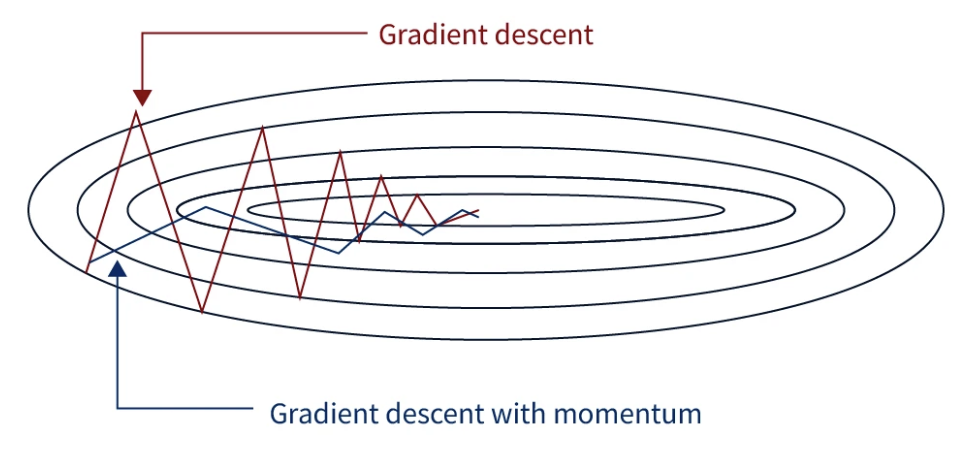
\includegraphics[scale=0.4]{figures/machine_learning/stochasticgradientdescent}
\caption{Stochastic Gradient Descent (SGD) Algorithm with and without Momentum}
\end{figure}

\begin{remark} \hlt{Nesterov Momentum}\\
Inspired by Nesterov's accelerated gradient method, the update rules are:
\begin{align}
\bm{v} &\leftarrow \alpha \bm{v} - \epsilon \nabla_{\bm{\theta}} \left(\frac{1}{m} \sum\limits_{i=1}^m L(\bm{f}(\bm{x}^{(i)}; \bm{\theta} + \alpha \bm{v}), \bm{y}^{(i)}) \right) \nonumber \\
\bm{\theta} &\leftarrow \bm{\theta} + \bm{v} \nonumber
\end{align}
Note, gradient is evaluated after current velocity is applied.\\
Hence, Nesterov momentum is adding a correction factor to the standard method of momentum.
\end{remark}

\begin{breakablealgorithm}
\caption{Stochastic Gradient Descent (SGD) with Nesterov Momentum}
\begin{algorithmic}
\Require \\
Learning rate $\epsilon_k$, Momentum parameter $\alpha$\\
Initial parameter $\bm{\theta}$, Initial velocity $\bm{v}$\\

\While {stopping criterion not met}
\State Sample a minibatch of $m$ samples from the training set $\{\bm{x}^{(1)}, \ldots, \bm{x}^{(m)} \}$ with targets $\bm{y}^{(i)}$
\State Apply interim update: $\tilde{\bm{\theta}} \leftarrow \bm{\theta} + \alpha \bm{v}$
\State Compute gradient (at interim point): $\bm{g} \leftarrow \frac{1}{m} \nabla_{\tilde{\bm{\theta}}} \sum_{i} L(f(\bm{x}^{(i)}; \tilde{\bm{\theta}}), \bm{y}^{(i)})$
\State Compute velocity update: $\bm{v} \leftarrow \alpha \bm{v} - \epsilon \bm{g}$
\State Apply update: $\bm{\theta} \leftarrow \bm{\theta} + \bm{v}$
\EndWhile
\end{algorithmic}
\end{breakablealgorithm}

\begin{figure}[H]
\centering
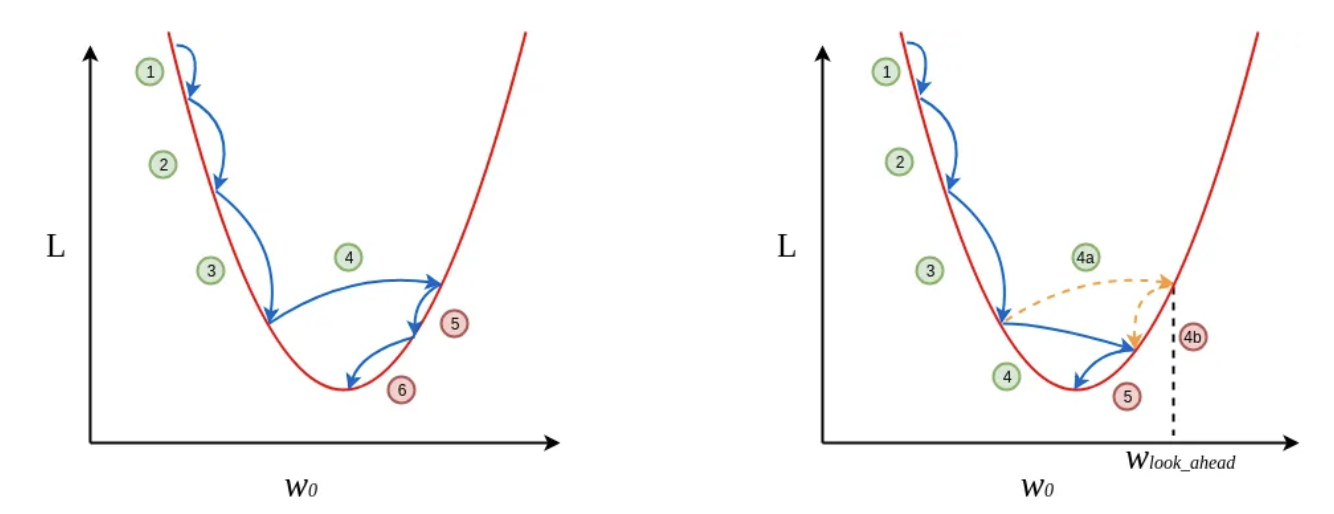
\includegraphics[scale=0.4]{figures/machine_learning/nesterov}
\caption{Momentum vs Nesterov Gradient Descent}
\end{figure}

\begin{remark} \hlt{Parameter Initialisation Challenges}\\
Training deep neural networks is difficult as most algorithms are strongly affected by choice of initialisation.\\
Designing initialisation strategies is difficult as neural network optimisation is not yet well understood, as the nice properties from initialisation may not be preserved as training proceeds.\\
Some initial points may be beneficial for optimisation, but detrimental for generalisation.
\end{remark}

\begin{remark} \hlt{Parameter Initialisation Strategies}\\
Initial parameters need to 'break symmetry' between different units. May explicitly search for large set of basis functions mutually different from each other, but this may incur noticeable computational cost.\\
Random initialisation from high-entropy distribution over high-dimensional space is computationally cheaper.\\
Larger initial weights will yield stronger symmetry breaking effect and avoid redundant units. However, if weights are set too large, may result in chaos (extreme sensitivity to small perturbations of input). Exploding gradient may be mitigated by gradient clipping. The bias (i.e., parameters encoding conditional variance of a prediction) for each unit is set to heuristically chosen constraints.
\end{remark}

\begin{remark} \hlt{Weight Initialisation Heuristics}\\
Initialising parameters of neural network $\bm{\theta}$ to $\bm{\theta}_0$ is similar to imposing a Gaussian prior $p(\bm{\theta})$ with mean $\bm{\theta}_0$, hence it make sense to choose $\bm{\theta}_0$ near $0$. Initialisation of $\bm{\theta}_0$ to large values means prior specifies which units should interact with each other, and how they should interact.\\
For a fully connected neural network with $m$ inputs and $n$ outputs, weights may be initialised by:
\begin{enumerate}[label=\roman*.]
\setlength{\itemsep}{0pt}
\item Sampling from $U\left(-\frac{1}{\sqrt{m}},  \frac{1}{\sqrt{m}} \right)$
\item Sampling from normalised initialisation $W_{i,j} \sim U \left(-\sqrt{\frac{6}{m+n}},  \sqrt{\frac{6}{m+n}} \right)$ (Glorot and Bengio). Compromise between goal of initialising all layers to have same activation variance and that of same gradient variance. Derived from assumption that network is chain of matrix multiplications with no nonlinearities.
\item Sampling from random orthogonal matrices, with scaling or gain factor $g$ that accounts for nonlinearity at each layer, with specific values for different types of nonlinear activation functions. Assumes neural network is sequence of matrix multiplications without nonlinearities. Guarantees the total number of training iterations required to reach convergence is independent of depth.\\
Increasing scaling factor $g$ pushes network toward regime where activations increase in norm in forward propagation, and gradients increase in norm in backward propagation.\\
For scaling rules that set all of initial weights to have same standard deviation, individual weight becomes extremely small when layers become large.
\item Sparse initialisation (Martens), where each unit is initialised to have exactly $k$ non-zero weight. Keep total number of input to unit independent from number of inputs $m$ without making magnitude of individual weight elements shrink with $m$.\\
Imposes very strong prior on weights that are chosen to have large Gaussian values.
\end{enumerate}
If computational resources allow, treat initial scale of weights for each layer as a hyper-parameter, and use hyper-parameter search algorithm. Choice of dense or sparse initialisation may also be a hyper-parameter.
\end{remark}

\begin{remark} \hlt{Bias Initialisation Heuristics}\\
Setting bias to zero is compatible with most weight initialisation schemes. The few other situations are:
\begin{enumerate}[label=\roman*.]
\setlength{\itemsep}{0pt}
\item If bias is for output unit, initialise bias to obtain right marginal statistics of the output. Assume initial weights are small enough that output of unit is determined only by bias. The bias will be inverse of activation function applied to marginal statistics of the output in training set.\\
If output is a highly skewed distribution over classes with marginal probability of class $i$ given by element $c_i$ of some vector $\bm{c}$, then bias vector $\bm{b}$ is such that $\text{softmax}(\bm{b}) = \bm{c}$. The models have output layers that should resemble input data $\bm{x}$, hence bias should match marginal distribution over $\bm{x}$.
\item If bias is to be set to avoid causing too much saturation at initialisation (i.e., with ReLU). Not compatible with weight initialisation schemes that do not expect strong input form bias (i.e., with random walk init).
\item If a unit controls whether other units are able to participate in a function. There is unit with output $u$ and another unit $h \in [0,1]$, multiplied together to produce output $uh$. Then $h$ is a gate that determines if $uh \approx u$ or $uh \approx 0$. Hence, to set bias for $h$ such that $h \approx 1$ at initialisation, else $u$ does not learn.
\end{enumerate}
\end{remark}

\begin{remark} \hlt{Variance or Precision Parameter Initialisation Heuristics}\\
For linear regression with conditional variance estimate using model
\begin{align}
p(y \ | \ \bm{x}) = \mathcal{N}(y \ | \ \bm{w}^T \bm{x} + b, 1/\beta) \nonumber
\end{align}
where $\beta$ is a precision parameter. The variance of precision parameters may be initialised to $1$.\\
Another approach is to assume initial weights are close enough to zero, and bias may be set while ignoring effect of the weights, then set bias to produce the correct marginal mean of the output, and set variance parameters to the marginal variance of the output in the training set.
\end{remark}

\begin{remark} \hlt{Model Parameter Initialisation with Machine Learning}\\
Initialise supervised model with parameters learned by unsupervised model trained on same inputs.\\
Alternatively, perform supervised training on a related task, which may yield initialisation that offers faster convergence than random initialisation. Information on distribution is encoded into initial parameters of model.
\end{remark}

\begin{remark} \hlt{Adaptive Gradient (AdaGrad) Algorithm}\\
Algorithm individually adapts learning rates of all model parameters by scaling them inversely proportional to square root of sum of all of their historical squared values. Has greater progress in more gently sloped directions of parameter space. On deep neural networks, accumulation of squared gradients from beginning of training can result in premature and excessive decrease in effective learning rate.
\end{remark}

\begin{breakablealgorithm}
\caption{Adaptive Gradient (AdaGrad) Algorithm}
\begin{algorithmic}
\Require \\
Global Learning rate $\epsilon$\\
Initial parameter $\bm{\theta}$\\
Small constant $\delta$, perhaps $10^{-7}$ for numerical stability\\

\State Initialise gradient accumulation variable $\bm{r} = \bm{0}$
\While {stopping criterion not met}
\State Sample a minibatch of $m$ samples from the training set $\{\bm{x}^{(1)}, \ldots, \bm{x}^{(m)} \}$ with targets $\bm{y}^{(i)}$
\State Compute gradient: $\bm{g} \leftarrow \frac{1}{m} \nabla_{\bm{\theta}} \sum_i L(f(\bm{x}^{(i)}; \bm{\theta}), \bm{y}^{(i)})$
\State Accumulate squared gradient: $\bm{r} \leftarrow \bm{r} + \bm{g} \odot \bm{g}$
\State Compute update: $\Delta \bm{\theta} \leftarrow - \frac{\epsilon}{\delta + \sqrt{\bm{r}}} \odot \bm{g}$ (Division and square root applied element-wise)
\State Apply update: $\bm{\theta} \leftarrow \bm{\theta} + \Delta \bm{\theta}$
\EndWhile
\end{algorithmic}
\end{breakablealgorithm}

\begin{remark} \hlt{Root Mean Squared Propagation (RMSProp) Algorithm}\\
Modifies AdaGrad to perform better in non-convex setting by changing gradient accumulation into exponentially weighted moving average, which discards history from extreme past so it can converge rapidly after finding a convex bowl. Use of moving average introduces a new hyper-parameter $\rho$ that controls length scale of the moving average. RMSProp is effective and practical for deep neural networks.
\end{remark}

\begin{breakablealgorithm}
\caption{Root Mean Squared Propagation (RMSProp) Algorithm}
\begin{algorithmic}
\Require \\
Global Learning rate $\epsilon$\\
Decay rate $\rho$\\
Initial parameter $\bm{\theta}$\\
Small constant $\delta$, perhaps $10^{-6}$ to stabilise division by small numbers\\

\State Initialise accumulation variable $\bm{r} = \bm{0}$
\While {stopping criterion not met}
\State Sample a minibatch of $m$ samples from the training set $\{\bm{x}^{(1)}, \ldots, \bm{x}^{(m)} \}$ with targets $\bm{y}^{(i)}$
\State Compute gradient: $\bm{g} \leftarrow \frac{1}{m} \nabla_{\bm{\theta}} \sum_i L(f(\bm{x}^{(i)}; \bm{\theta}), \bm{y}^{(i)})$
\State Accumulate squared gradient: $\bm{r} \leftarrow \rho \bm{r} + (1 - \rho) \bm{g} \odot \bm{g}$
\State Compute update: $\Delta \bm{\theta} \leftarrow - \frac{\epsilon}{\sqrt{\delta + \bm{r}}} \odot \bm{g}$ ($\frac{\epsilon}{\sqrt{\delta + \bm{r}}}$ applied element-wise)
\State Apply update: $\bm{\theta} \leftarrow \bm{\theta} + \Delta \bm{\theta}$
\EndWhile
\end{algorithmic}
\end{breakablealgorithm}

\begin{breakablealgorithm}
\caption{Root Mean Squared Propagation (RMSProp) Algorithm}
\begin{algorithmic}
\Require \\
Global Learning rate $\epsilon$\\
Decay rate $\rho$\\
Momentum coefficient $\alpha$\\
Initial parameter $\bm{\theta}$\\
Initial velocity $\bm{v}$\\

\State Initialise accumulation variable $\bm{r} = \bm{0}$
\While {stopping criterion not met}
\State Sample a minibatch of $m$ samples from the training set $\{\bm{x}^{(1)}, \ldots, \bm{x}^{(m)} \}$ with targets $\bm{y}^{(i)}$
\State Compute interim update $\tilde{\bm{\theta}} \leftarrow \bm{\theta} + \alpha \bm{v}$
\State Compute gradient: $\bm{g} \leftarrow \frac{1}{m} \nabla_{\tilde{\bm{\theta}}} \sum_i L(f(\bm{x}^{(i)}; \tilde{\bm{\theta}}), \bm{y}^{(i)})$
\State Accumulate gradient: $\bm{r} \leftarrow \rho \bm{r} + (1 - \rho) \bm{g} \odot \bm{g}$
\State Compute velocity update: $\bm{v} \leftarrow \alpha \bm{v} - \frac{\epsilon}{\sqrt{\bm{r}}} \odot \bm{g}$ ($\frac{1}{\sqrt{\bm{r}}}$ applied element-wise)
\State Apply update: $\bm{\theta} \leftarrow \bm{\theta} + \bm{v}$
\EndWhile
\end{algorithmic}
\end{breakablealgorithm}

\begin{remark} \hlt{Adaptive Moment Estimation (Adam) Algorithm}\\
Variant on combination of RMSProp and momentum. Note, momentum is incorporated directly as an estimate of first order moment of gradient; bias corrections are made to estimates of both first-order moments and second-order moments to account for initialisation at origin.\\
Algorithm is fairly robust to choice of hyper-parameters.
\end{remark}

\begin{breakablealgorithm}
\caption{Adaptive Moment Estimation (Adam) Algorithm}
\begin{algorithmic}
\Require \\
Step size $\epsilon$ (Suggested default: $0.001$)\\
Exponential decay rates for moment estimates $\rho_1, \rho_2$ in $[0,1)$ (Suggested defaults: $0.9$ and $0.999$)\\
Small constant $\delta$ used for numerical stabilisation (Suggested default: $10^{-8}$)\\
Initial parameters $\bm{\theta}$\\

\State Initialise $1$st and $2$nd momentum variables $\bm{s} = \bm{0}$, $\bm{r} = \bm{0}$
\State Initialise time step $t=0$
\While {stopping criterion not met}
\State Sample a minibatch of $m$ samples from the training set $\{\bm{x}^{(1)}, \ldots, \bm{x}^{(m)} \}$ with targets $\bm{y}^{(i)}$
\State Compute gradient: $\bm{g} \leftarrow \frac{1}{m} \nabla_{\bm{\theta}} \sum_i L(f(\bm{x}^{(i)}; \bm{\theta}), \bm{y}^{(i)})$
\State Update time step $t \leftarrow t+1$
\State Update biased first and second moment estimate: $\bm{s} \leftarrow \rho_1 \bm{s} + (1-\rho_1) \bm{g}$ and $\bm{r} \leftarrow \rho_2 \bm{r} + (1-\rho_2) \bm{g} \odot \bm{g}$
\State Correct bias in first and second moment: $\hat{\bm{s}} \leftarrow \frac{\bm{s}}{1 - \rho_1^t}$ and $\hat{\bm{r}} \leftarrow \frac{\bm{r}}{1 - \rho_2^t}$
\State Compute update: $\Delta \bm{\theta} = - \epsilon \frac{\hat{\bm{s}}}{\sqrt{\hat{\bm{r}} + \delta}}$ (Operations applied element-wise)
\State Apply update: $\bm{\theta} \leftarrow \bm{\theta} + \Delta \bm{\theta}$
\EndWhile
\end{algorithmic}
\end{breakablealgorithm}

\begin{remark} \hlt{Newton's Method}\\
Based on second-order Taylor's series approximating $J(\bm{\theta})$ near the point $\bm{\theta}_0$, ignoring higher derivatives
\begin{equation*}
J(\bm{\theta}) \approx J(\bm{\theta}_0) + (\bm{\theta} - \bm{\theta}_0)^T \nabla_{\bm{\theta}} J(\bm{\theta}_0) + \frac{1}{2} (\bm{\theta} - \bm{\theta}_0)^T \bm{H}(\bm{\theta} - \bm{\theta}_0) \nonumber
\end{equation*}
where $\bm{H}$ is the Hessian of $J$ with respect to $\bm{\theta}$ evaluated at $\bm{\theta}_0$.\\
Solving for critical point will get the Newton parameter update rule
\begin{equation*}
\bm{\theta}^{*} = \bm{\theta}_0 - \bm{H}^{-1} \nabla_{\bm{\theta}} J(\bm{\theta}_0) \nonumber
\end{equation*}
Note that for deep learning, the surface of objective function is non-convex. Regularising the Hessian will solve many of the issues such as saddle points etc.
\begin{equation*}
\bm{\theta}^{*} = \bm{\theta}_0 - [H(f(\bm{\theta}_0)) + \alpha \bm{I}]^{-1} \nabla_{\bm{\theta}} J(\bm{\theta}_0) \nonumber
\end{equation*}
Due to requirement for inversion of the $k \times k$ matrix with time complexity $O(k^3)$ at every training iteration, only networks with very small number of parameters may be trained with this method.
\end{remark}

\begin{breakablealgorithm}
\caption{Newton's Method with Objective $J(\bm{\theta}) = \frac{1}{m} \sum_{i=1}^m L(f(\bm{x}^{(i)}; \bm{\theta}), y^{(i)})$}
\begin{algorithmic}
\Require \\
Initial parameter $\bm{\theta}_0$\\
Training set of $m$ examples\\

\While {stopping criterion not met}
\State Compute gradient $\bm{g} \leftarrow \frac{1}{m} \nabla_{\bm{\theta}} \sum_i L(f(\bm{x}^{(i)}; \bm{\theta}), \bm{y}^{(i)})$
\State Compute Hessian: $\bm{H} \leftarrow \frac{1}{m} \nabla_{\bm{\theta}}^2 \sum_i L(f(\bm{x}^{(i)}; \bm{\theta}), \bm{y}^{(i)})$
\State Compute Hessian Inverse: $\bm{H}^{-1}$
\State Compute update: $\Delta \bm{\theta} = - \bm{H}^{-1} \bm{g}$
\State Apply update: $\bm{\theta} \leftarrow \bm{\theta} + \Delta \bm{\theta}$
\EndWhile
\end{algorithmic}
\end{breakablealgorithm}

\begin{remark} \hlt{Conjugate Gradient Method}\\
Method effectively avoids computation of inversion Hessian by descending conjugate directions, which is a search direction conjugate to the previous line search direction (will not undo progress made in that direction).\\
Let current and previous search directions be $\bm{d}_{t}, \bm{d}_{t-1}$. At training iteration $t$, the next search direction $\bm{d}_t$ is
\begin{equation*}
\bm{d}_t = \nabla_{\bm{\theta}} J(\bm{\theta}) + \beta_t \bm{d}_{t-1} \nonumber
\end{equation*}
note that $\beta_t$ may be computed via Fletcher Reeves:
\begin{equation*}
\beta_t = \frac{\nabla_{\bm{\theta}} J(\bm{\theta}_t)^T \nabla_{\bm{\theta}} J(\bm{\theta}_t)}{\nabla_{\bm{\theta}} J(\bm{\theta}_{t-1})^T \nabla_{\bm{\theta}} J(\bm{\theta}_{t-1})} \nonumber
\end{equation*}
or may be computed with Polak-Ribiere:
\begin{equation*}
\beta_t = \frac{(\nabla_{\bm{\theta}} J(\bm{\theta}_t) - \nabla_{\bm{\theta}} J(\bm{\theta}_{t-1}))^T \nabla_{\bm{\theta}} J(\bm{\theta}_t)}{\nabla_{\bm{\theta}} J(\bm{\theta}_{t-1})^T \nabla_{\bm{\theta}} J(\bm{\theta}_{t-1})} \nonumber
\end{equation*}
The non-linear conjugate gradient method is a variation which uses occasional resets where the method is restarted with line search along with the unaltered gradient.
\end{remark}

\begin{breakablealgorithm}
\caption{Conjugate Gradient Method}
\begin{algorithmic}
\Require \\
Initial parameter $\bm{\theta}_0$\\
Training set of $m$ examples\\
Initialise $\bm{\rho}_0 = 0$\\
Initialise $g_0 = 0$\\
Initialise $t = 1$\\

\While {stopping criterion not met}
\State Initialise the gradient $\bm{g}_t = \bm{0}$
\State Compute gradient $\bm{g} \leftarrow \frac{1}{m} \nabla_{\bm{\theta}} \sum_i L(f(\bm{x}^{(i)}; \bm{\theta}), \bm{y}^{(i)})$
\State Compute Polak-Ribiere metric: $\beta_t = \frac{(\bm{g}_t - \bm{g}_{t-1})^T \bm{g}_t}{\bm{g}_{t-1}^T \bm{g}_{t-1}}$
\State (Nonlinear conjugate gradient: optionally reset $\beta_t = 0$, i.e., if $t$ is a multiple of some constant $k$)
\State Compute search direction: $\bm{\rho}_t = -\bm{g}_t + \beta_t \bm{\rho}_{t-1}$
\State Perform line search to find: $\epsilon^{*} = \arg \min_{\epsilon} \frac{1}{m} \sum_{i=1}^m L(f(\bm{x}^{(i)}; \bm{\theta}_t + \epsilon \bm{\rho}_t), \bm{y}^{(i)})$
\State (On truly quadratic cost function, analytically solve for $\epsilon^{*}$)
\State Apply update: $\bm{\theta}_{t+1} = \bm{\theta}_{t} + \epsilon^{\theta} \bm{\rho}_t$
\State Apply time step $t \leftarrow t + 1$
\EndWhile
\end{algorithmic}
\end{breakablealgorithm}

\begin{remark} \hlt{Nonlinear Conjugate Gradients}\\
Method of conjugate gradients is still applicable for non-linear objective function.\\
Conjugate directions are no longer assumed to remain at minimum of the objective for previous directions. Has occasional resets where method of conjugate gradients is restarted with line search along unaltered gradient.
\end{remark}

\begin{remark} \hlt{Broyden-Fletcher-Goldfarb-Shanno (BGFS) Algorithm}\\
Similar to conjugate gradient, but uses more direct approach to approximation of newton's update.\\
Method approximate the inverse of hessian $\bm{H}$ with matrix $\bm{M}_t$, iteratively refined by low rank updates to better approximate $\bm{H}^{-1}$. Direction of gradient descent is then determined by $\bm{\rho}_t = \bm{M}_t \bm{g}_t$. Line search is performed in this direction to determine step size $\epsilon^{*}$. Final update of parameter is then $\bm{\theta}_{t+1} = \bm{\theta}_t + \epsilon^{*} \bm{\rho}_{t}$.\\
Note, BGFS store matrix $\bm{M}$ which requires $O(n^2)$ memory, making it impractical for most modern models.
\end{remark}

\begin{remark} \hlt{Limited Memory BFGS (L-BFGS) Algorithm}\\
Memory costs of BFGS may be decreased by not storing complete inverse Hessian approximation $\bm{M}$. L-BFGS computes approximation $\bm{M}$ with same method as BFGS, but assumes at beginning that $\bm{M}^{(t-1)}$ is the identity matrix, rather than storing the approximation between steps.\\
If used with exact line searches, directions defined by L-BFGS are mutually conjugate, and this procedure remains well-behaved when minimum of line search is reached only approximately.\\
L-BFGS may be generalised to store some vectors used to update $\bm{M}$ at each time step, costing $O(n)$ per step.
\end{remark}

\begin{remark} \hlt{Meta-Algorithm: Batch Normalisation}\\
An update from optimisation algorithm may result in multiple-order effects, and in very deep networks, even higher-order interactions can be significant.\\
Batch normalisation provides an elegant way of re-parametrising any deep network, which reduces the problem of coordinating updates across multiple layers. Batch normalisation may be applied to any input/hidden layer.\\
Let $\bm{H}$ be minibatch of activations of layer to normalise, with activations for each example appearing in a row. To normalise $\bm{H}$, replace it with $\bm{H}' = \frac{\bm{H} - \bm{\mu}}{\bm{\sigma}}$ where $\bm{\mu}$ is a vector of mean of each unit and $\sigma$ is a vector of standard deviation of each unit. Then $H_{ij}$ is normalised by subtracting $\mu_j$ and dividing $\sigma_j$. Rest of network then operates on $\bm{H}'$ just as in original network on $\bm{H}$.\\
At training, the mean and standard deviations are computed as
\begin{align}
\bm{\mu} &= \frac{1}{m} \sum\limits_i \bm{H}_{i, ;}, \ \ \ \bm{\sigma} = \sqrt{\delta + \frac{1}{m} \sum\limits_{i} (\bm{H} - \bm{\mu})^2_i} \nonumber
\end{align}
where $\delta$ is a small positive value (i.e., $10^{-8}$) to avoid undefined gradient of $\sqrt{z}$ at $z=0$.\\
These are then back-propagated to normalise $\bm{H}$, hence gradient will never increase the standard deviation or mean of $h_i$. Batch normalisation re-parametrises the model to make some units always standardised.\\
At test time, $\mu$ and $\sigma$ may be replaced by running averages from training time. This allows model to be evaluated on a single example, without needing to use definitions of $\mu$ and $\bm{\sigma}$ that depends on entire minibatch.
\end{remark}

\begin{remark} \hlt{Batch Normalisation but Maintain Network Express Power}\\
Replace batch of hidden activations $\bm{H}$ with $\bm{\gamma} \bm{H}' + \bm{\beta}$ rather than $\bm{H}'$, where $\bm{\gamma}$ and $\bm{\beta}$ are learned parameters to allow new variable to have any mean and standard deviation. With original $\bm{H}'$, mean of $\bm{H}$ was determined by complicated interaction between parameters in layers below $\bm{H}$. With $\bm{\gamma} \bm{H}' + \bm{\beta}$, the mean is determined solely by $\bm{\beta}$, which is much easier to learn with gradient descent.\\
Most neural network layers are of form $\phi(\bm{X} \bm{W} + \bm{b})$, where $\phi$ is some fixed nonlinear activation function. Then $\bm{X} \bm{W} + \bm{b})$ should be replaced by normalised version of $\bm{X} \bm{W}$, and bias term omitted as it becomes redundant with $\beta$ parameter applied from batch normalisation re-parametrisation. Statistics of input are non-Gaussian and less amenable to standardisation by linear operations.	
\end{remark}

\begin{remark} \hlt{Meta-Algorithm: Coordinate Descent}\\
Solving optimisation problems by minimising the objective function $f(\bm{x})$ with respect to a single variable $x_i$, and rapidly cycling through all variables. \hlt{Block coordinate descent} refers to minimising with respect to a subset of variables simultaneously.\\
 Coordinate descent works when different variables can be clearly separated into groups that play relatively isolated roles, or when optimisation with respect to one group of variables is significantly more efficient than optimisation with respect to all of the variables.
\end{remark}

\begin{example} \hlt{Sparse Encoding with Coordinate Descent}\\
Consider the cost function
\begin{align}
J(\bm{H}, \bm{W}) = \sum\limits_{i,j} \abs{H_{ij}} + \sum\limits_{i,j} (\bm{X} - \bm{W}^T \bm{H})^2_{i,j} \nonumber
\end{align}
To find weight matrix $\bm{W}$ that can linearly decode a matrix of activation values $\bm{H}$ to reconstruct training set $\bm{X}$. Most applications also include weight decay or constraint on norms of columns of $\bm{W}$ to prevent the pathological solution with extremely small $\bm{H}$ and large $\bm{W}$.\\
Note $J$ is not convex, but inputs may be divided into the dictionary parameters $\bm{W}$ and the code representations $\bm{H}$. Minimising object function with respect to either set is a convex problem.
\end{example}

\begin{remark} \hlt{Polyak Averaging}\\
Average several points in trajectory through parameter space visited by optimisation algorithm.\\
If $t$ iterations of gradient descent visit points $\bm{\theta}^{(1)}, \ldots, \bm{\theta}^{(t)}$, then the output is $\hat{\bm{\theta}}^{(t)} = \frac{1}{t} \sum_i \bm{\theta}^{(i)}$.\\
The optimisation algorithm may leap back and forth across a valley several times without visiting the minimum point, and the average of all points on either side of the valley should be close to minimum value.\\
This is developed solely for stochastic gradient descent (SGD) to stabilise the estimates (\cite{granziol2020gadam}).\\
For non-convex problems, an exponentially decaying running average is used:
\begin{align}
\hat{\bm{\theta}}^{(t)} = \alpha \hat{\bm{\theta}}^{(t-1)} + (1- \alpha)\bm{\theta}^{(t)} \nonumber
\end{align}
\end{remark}

\begin{remark} \hlt{Supervised Pre-training}\\
Pre-training refers to training simple models on simple tasks before training the desired model on desired task.\\
Greedy algorithms break problem into many components, then solve for optimal version of each component in isolation, which is must cheaper than algorithms that solve for best joint solution. Fine-tuning on joint optimisation algorithm searches for optimal solution to the full problem.\\
Greedy supervised training breaks supervised learning problems into other simpler supervised learning problems.\\
Transfer learning refers to pre-training a deep network on a set of tasks, then initialise a same-size network with first $k$ layers of first net. The layers of second networks (upper layers initialised randomly) are then jointly trained to perform a different set of tasks with fewer training examples than for first set of tasks.\\
FitNets approach begins by training a network with low depth and high width, which becomes a teacher for a second network (the student), which is much deeper and thinner. Student network is trained to not only predict the output on original task, but also on value of middle layer of teacher network.
\end{remark}

\begin{remark} \hlt{Neural Network Design Choice: Linear Transformation}\\
Model units have generally moved towards using more linear functions, which allow model to have nice properties that make optimisation easier. The model's local gradient information corresponds reasonably well to moving towards a distant solution.
\end{remark}

\begin{remark} \hlt{Neural Network Design Choice: Linear Paths and Skip Connections}\\
Linear paths and skip connections between layers reduce length of shortest path from lower layer's parameters to the output, mitigating vanishing gradient problem.\\
Adding extra copies of output that are attached to intermediate hidden layers is an alternative to pre-training, where these 'auxiliary heads' are trained to perform the same task as primary output at the top of the network to ensure that the lower layers receive a large gradient. After training, these may be discarded.
\end{remark}

\begin{remark} \hlt{Continuation Methods}\\
Family of strategies that can make optimisation easier by choosing initial points to ensure that local optimisation spends most of its time in well-behaved regions. Method constructs series of objective functions $\{J^{(0)}, \ldots, J^{(n)}\}$ which are increasingly difficult to minimise (well-behaved over less regions of $\bm{\theta}$ space) for the true cost function $J(\bm{\theta})$. The cost functions are designed such that a solution to one is a good initial point for the next.\\
Continuation methods aim to reach a global minimum despite many local minima. Easier cost functions are constructed through the blurring operation, which approximates
\begin{align}
J^{(i)}(\bm{\theta}) = \mathbb{E}_{\theta' \sim \mathcal{N}(\bm{\theta}'; \bm{\theta}, \sigma^{(i)2})} J(\bm{\theta})' \nonumber
\end{align}
via sampling. Some non-convex functions become approximately convex when blurred, but preserved enough information about local global minimum. However, approach might not work when
\begin{enumerate}[label=\roman*.]
\setlength{\itemsep}{0pt}
\item so many incremental cost functions are required that cost of entire procedure remains high;
\item NP-hard optimisation problems remain NP-hard, even when continuation methods are applicable;
\item function might not become convex, no matter how much it is blurred;
\item function may become convex due to blurring, but minimum of this blurred function may track a local rather than global minimum of original cost function.
\end{enumerate}
\end{remark}

\begin{remark} \hlt{Curriculum Learning}\\
Planning a learning process to begin by learning simple concepts, and progress to learning more complex topics that depend on these simpler concepts. Earlier objective functions $J^{(i)}$ are made easier by increasing the influence of simpler examples.\\
Stochastic curriculum is a variation of the approach where a random mix of easy and difficult examples is always presented to the learner, but average proportion of more difficult examples is gradually increased.
\end{remark}


\subsection{Regularization and Generalization}
% Dropout, weight decay, data augmentation, implicit regularization, scaling behavior.

\subsection{Regularisation for Deep Learning}

\begin{definition} \hlt{Regularisation} refers to adding a parameter norm penalty $\Omega(\bm{\theta})$ to the objective function $J$. The regularised objective function is then
\begin{equation*}
\tilde{J}(\bm{\theta}; \bm{X}, \bm{y}) = J(\bm{\theta}; \bm{X}, \bm{y}) + \alpha \Omega(\bm{\theta}) \nonumber
\end{equation*}
where $\alpha in [0, \infty)$ is a hyper-parameter that weights the contribution of norm penalty term.\\
For neural networks, the parameter norm penalty $\Omega$ is chosen such that it penalises only the weights of the affine transformation at each layer and leaves the biases un-regularised.
\end{definition}

\begin{definition} \hlt{$L^2$ (Ridge) Regularisation}\\
The regularisation term added to objective function is
\begin{equation*}
\Omega(\bm{\theta}) = \frac{1}{2} \Vert \bm{w} \Vert^2_2 \nonumber
\end{equation*}
\end{definition}

\begin{remark} \hlt{Behaviour of Weight Decay ($L^2$) Regularisation}\\
Assuming no bias parameter, a model have the following objective function and parameter gradient:
\begin{align*}
\tilde{J}(\bm{w}; \bm{X}, \bm{y}) &= \frac{\alpha}{2} \bm{w}^T \bm{w} + J(\bm{w}; \bm{X}, \bm{y}) \nonumber \\
\nabla_{\bm{w}} \tilde{J}(\bm{w}; \bm{X}, \bm{y}) &= \alpha \bm{w} + \nabla_{\bm{w}} J(\bm{w}; \bm{X}, \bm{y}) \nonumber
\end{align*}
On a single gradient step, the update is as follows:
\begin{align*}
\bm{w} \leftarrow (1 - \epsilon \alpha)\bm{w} - \epsilon \nabla_{\bm{w}} J(\bm{w}; \bm{X}, \bm{y}) \nonumber
\end{align*}
The addition of weight decay has modified learning rule to multiplicatively shrink weight vector by constant factor on each step before gradient update.\\
Using quadratic approximation to objective function at minimal unregularised training cost, approximation is
\begin{equation*}
\hat{J}(\overline{\theta}) = J(\bm{w}^*) + \frac{1}{2} (\bm{w} - \bm{w}^*)\bm{H}(\bm{w} - \bm{w}^*), \ \ \ \ \bm{w}^* = \arg \min_{\bm{w}} J(\bm{w}) \nonumber
\end{equation*}
where $\bm{H}$ is Hessian matrix of $J$ with respect to $\bm{w}$ evaluated at $\bm{w}^*$. Minimum of $\hat{J}$ occurs where gradient is
\begin{align}
\nabla_{\bm{w}} \hat{J}(\bm{w}) = \bm{H}(\bm{w} - \bm{w}^*) = \bm{0} \nonumber
\end{align}
Adding weight decay gradient, solve for minimum of regularised version of $\hat{J}$. Let $\tilde{\bm{w}}$ be minimum, then
\begin{align}
\alpha \tilde{\bm{w}} + \bm{H}(\tilde{\bm{w}} - \bm{w}^*) = 0 \nonumber \\
(\bm{H} + \alpha \bm{I})\tilde{\bm{w}} = \bm{H} \bm{w}^* \nonumber \\
\tilde{\bm{w}} = (\bm{H} + \alpha \bm{I})^{-1} \bm{H} \bm{w}^* \nonumber
\end{align}
As $\alpha \rightarrow 0$, regularised solution $\tilde{\bm{w}} \rightarrow \bm{w}^*$. Note $\bm{H}$ is real and symmetric, hence decompose into diagonal matrix $\bm{A}$ and orthonormal basis of eigenvectors $\bm{Q}$ such that $\bm{H} = \bm{Q} \bm{\Lambda} \bm{Q}^T$, to get
\begin{equation*}
\tilde{\bm{w}} = (\bm{Q} \bm{\Lambda} \bm{Q}^T + \alpha \bm{I})^{-1} \bm{Q} \bm{\Lambda} \bm{Q}^T \bm{w}^* = \bm{Q} (\bm{\Lambda} + \alpha \bm{I})^{-1} \bm{\Lambda} \bm{Q}^T \bm{w}^* \nonumber
\end{equation*}
The effect of weight decay rescale $\bm{w}^*$ along axes defined by eigenvectors of $\bm{H}$. The component of $\bm{w}^*$ aligned with $i$-th eigenvector of $\bm{H}$ is rescaled by factor $\frac{\lambda_i}{\lambda_i + \alpha}$. For components where $\lambda_i \gg \alpha$, the effects of regularisation is relatively small. For components where $\lambda_i \ll \alpha$, components will be shrunk to nearly zero magnitude.
\end{remark}

\begin{definition} \hlt{$L^1$ Regularisation}\\
The $L^1$ regularisation is the sum of absolute values of individual parameters.
\begin{equation*}
\Omega(\bm{\theta}) = \Vert \bm{w} \Vert_1 = \sum_i \abs{w_i} \nonumber
\end{equation*}
\end{definition}

\begin{definition} \hlt{Behaviour of $L^1$ Regularisation}\\
Assuming no bias parameter, a model has the following objective function and parameter gradient:
\begin{align}
\tilde{J}(\bm{w}; \bm{X}, \bm{y}) &= \alpha \Vert \bm{w} \Vert_1 + J(\bm{w}; \bm{X}, \bm{y}) \nonumber \\
\nabla_{\bm{w}} \tilde{J}(\bm{w}; \bm{X}, \bm{y}) &= \alpha \ \text{sign}(\bm{w}) + \nabla_{\bm{w}} J(\bm{w}; \bm{X}, \bm{y}) \nonumber
\end{align}
Note that the regularisation contribution to gradient is a constant factor with sign equal to $\text{sign}(w_i)$. Minimum of $\tilde{J}$ occurs at where
\begin{equation*}
\nabla_{\bm{w}} \tilde{J}(\bm{w}) = \bm{H} (\bm{w} - \bm{w}^*) \nonumber
\end{equation*}
Assuming the Hessian is diagonal, $\bm{H} = \text{diag}([H_{1,1}, \ldots, H_{n,n}])$, where each $H_{i,i} > 0$. The quadratic approximation of regularised objective function is then
\begin{align}
\tilde{J}(\bm{w}; \bm{X}, \bm{y}) &= J(\bm{w}^*; \bm{X}, \bm{y}) + \sum_i \left[ \frac{1}{2} H_{i,i} (\bm{w}_i - \bm{w}_i^*)^2 + \alpha \abs{w_i} \right] \nonumber \\
w_i &= \text{sign}(w_i^*) \max \left\{ \abs{w_i^*} - \frac{\alpha}{H_{i,i}}, 0 \right\} \nonumber
\end{align}
For the case where $w_i^* > 0$ for all $i$, then
\begin{enumerate}[label=\roman*.]
\setlength{\itemsep}{0pt}
\item if $w_i^* \leq \frac{\alpha}{H_{i,i}}$, the optimal value is $w_i = 0$ as contribution of $J(\bm{w}; \bm{X}, \bm{y})$ to regularised objective $\tilde{J}(\bm{w}; \bm{X}, \bm{y})$ is overwhelmed in direction $i$ by $L^1$ regularisation which pushes $w_i$ to zero.
\item if $w_i^* > \frac{\alpha}{H_{i,i}}$, regularisation shifts optimal value of $w_i$ in the direction by $\frac{\alpha}{H_{i,i}}$.
\end{enumerate}
For the case where $w_i^* < 0$, this happens similarly, but with $L^1$ penalty decreasing $w_i$ by $\frac{\alpha}{H_{i,i}}$, with min value $0$.\\
Note that $L^1$ produces a more sparse solution, which is a feature selection mechanism.
\end{definition}

\begin{remark} \hlt{Norm Penalties as Constrained Optimisation}\\
Let cost function regularised by parameter norm penalty be
\begin{equation*}
\tilde{J}(\bm{\theta}; \bm{X}, \bm{y}) = J(\bm{\theta}; \bm{X}, \bm{y}) + \alpha \Omega(\bm{\theta}) \nonumber
\end{equation*}
Construct a generalised generalised Lagrange function,
\begin{equation*}
\mathcal{L}(\bm{\theta}; \bm{X}, \bm{y}) = J(\bm{\theta}; \bm{X}, \bm{y}) + \alpha (\Omega(\bm{\theta}) - k) \nonumber
\end{equation*}
The solution to the constrained problem is then
\begin{equation*}
\bm{\theta}^* = \arg \min_{\bm{\theta}} \max_{\alpha, \alpha \geq 0} \mathcal{L} (\bm{\theta}, \alpha) \nonumber
\end{equation*}
Note that optimal value $\alpha^*$ will shrink $\Omega(\bm{\theta})$, but not such that it is less than $k$.\\
Fixing $\alpha^*$, the problem is then a function of $\bm{\theta}$,
\begin{equation*}
\bm{\theta}^* = \arg \min_{\bm{\theta}} \mathcal{L} (\bm{\theta}, \alpha^*) = \arg \min_{\bm{\theta}} J(\bm{\theta}; \bm{X}, \bm{y}) + \alpha^* \Omega (\bm{\theta}) \nonumber
\end{equation*}
This is the regularised training problem of minimising $\tilde{J}$. The parameter norm penalty is imposing a constraint on the weights. If explicit constraints are to be used rather than penalties, use stochastic gradient descent on $J(\bm{\theta})$, then take the projected $\bm{\theta}$ to the nearest point that satisfies $\Omega(\bm{\theta}) < k$. This method is used if $k$ is predefined by user, and time is not to be spent on searching for $\alpha$ value that corresponds to this $k$.\\
Explicit constraints and re-projection work better in circumstances where non-convex optimisation is involved, and this may avoid getting stuck in local minima. Explicit constraints also impose stability, and together with high learning rate allows rapid exploration of parameter space.
\end{remark}

\begin{remark} \hlt{Dataset Augmentation}\\
Effective technique for object classification. Operations such as translation of images by few pixels in each direction can greatly improved generalisation, even if the model has been designed to be partially translation invariant using convolution and pooling techniques. Rotation and scaling of images are also quite effective.\\
For speech recognition tasks, noice injection will improve performance. To improve robustness, train models with random noise applied to inputs. Noise injection also works when applied to the hidden units (data augmentation at multiple levels of abstraction). Enabling dropout constructs new inputs by multiplying by noise.
\end{remark}

\begin{remark} \hlt{Noise Robustness}\\
For some models, addition of noise with infinitesimal variance at input of model is equivalent to imposing penalty on norm of the weights. Generally, noise injection can be much more powerful than simply shrinking the parameters, especially when noise is added to hidden units.\\
Noise may also be added to weights, which is primarily used in recurrent neural networks. This is a stochastic implementation of Bayesian inference over the weights (model weights are uncertain and representable via a probability distribution that reflects this uncertainty).\\
Adding noise to weights may also result in more stability in function to be learned. Let the cost function be 
\begin{align}
J = \mathbb{E}_{p(x,y)}[(\hat{y}(\bm{x}) - y)^2] \nonumber
\end{align}
where $\hat{y}(\bm{x})$ is function to be trained that maps set of features $\bm{x}$ to a scalar using least-squares cost function $J$.\\
Assume each input presentation include a random perturbation $\epsilon_{\bm{W}} \sim \mathcal{N}(\bm{\epsilon}; \bm{0}, \eta \bm{I})$ in the network weight of a standard $l$-layer MLP. Let the perturbed model be $\hat{y}_{\bm{\epsilon}_{\bm{W}}}(\bm{x})$. With injection o noise, objective function becomes
\begin{align}
\tilde{J}_{\bm{W}} &= \mathbb{E}_{p(\bm{x}, y, \bm{\epsilon}_{\bm{W}})}\left[(\hat{y}_{\bm{\epsilon}_{\bm{W}}}(\bm{x}) - y)^2 \right] = \mathbb{E}_{p(\bm{x}, y, \bm{\epsilon}_{\bm{W}})} \left[\hat{y}^2_{\bm{\epsilon}_{\bm{W}}}(\bm{x}) - 2 y \hat{y}_{\bm{\epsilon}_{\bm{W}}} + y^2 \right] \nonumber
\end{align}
For small $\eta$, the minimisation of $J$ with added noise (with covariance $\eta \bm{I}$) is equivalent to minimisation of $J$ with additional regularisation term $\eta \mathbb{E}_{p(\bm{x}), y} [\norm{\nabla_{\bm{W}} \hat{y}(\bm{x})}^2]$. This encourages parameters to go to regions of parameter space where small perturbations of weights have relatively small influence on output.
\end{remark}

\begin{remark} \hlt{Label Smoothing}\\
Datasets may have some mistake in $y$ labels. Regularise a model based on softmax with $k$ output values by replacing hard $0$ and $1$ classification targets with targets of $\frac{\epsilon}{k-1}$ and $1-\epsilon$ respectively, assuming that the training set label $y$ is correct with probability $1- \epsilon$. Cross-entropy can then be used on these soft targets.
\end{remark}

\begin{remark} \hlt{Semi-Supervised Learning}\\
Unlabelled examples $P(\bm{x})$ and $P(\bm{x}, \bm{y})$ are used to estimate $P(\bm{y} \ | \ \bm{x})$ or predict $\bm{y}$ from $\bm{x}$.\\
Construct a generative model of either $P(\bm{x})$ or $P(\bm{x}, \bm{y})$ which shares parameters with a discriminative model of $P(\bm{y} \ | \ \bm{x})$. The supervised criterion $\log P(\bm{y} \ | \ \bm{x})$ may then be traded with the unsupervised or generative one ($\log P(\bm{x})$ or $\log P(\bm{x}, \bm{y})$). The generative criterion then expresses a particular form of prior belief about the solution to the supervised learning problem (structure of $P(\bm{x})$ is connected to structure of $P(\bm{y} \ | \ \bm{x})$ such that is is captured by the shared parametrisation).
\end{remark}

\begin{remark} \hlt{Multi-Task Learning}\\
Improve generalisations by pooling examples (soft constraints imposed on parameters) from several tasks.\\
Different supervised tasks (predicting $\bm{y}^{(i)}$ given $\bm{x}$) share the same input $\bm{x}$, as well as some intermediate-level representation $\bm{h}^{(\text{shared})}$ capturing a common pool of factors. Model can be divided in two parts:
\begin{enumerate}[label=\roman*.]
\setlength{\itemsep}{0pt}
\item Task-specific parameters
\item Generic parameters, shared across all the tasks
\end{enumerate}
Improved generalisation and associated error bounds can be achieved due to shared parameters, but this only happens if some assumptions about statistical relationship between different tasks are valid.
\end{remark}

\begin{remark} \hlt{Early Stopping}\\
To obtain a model with better validation set error by returning to the parameter setting at the point in time with lowest validation set error. Model validation is done in parallel to model training.\\
Early stopping has the effect of restricting the optimisation procedure to a relatively small volume of parameter space in neighbourhood of initial parameter value $\bm{\theta}_o$. Assume $\tau$ optimisation steps are taken with learning rate $\epsilon$. The product $\epsilon \tau$ is a measure of effective capacity. Assuming gradient is bounded, restricting $\epsilon \tau$ limits the volume of parameter space reachable from $\bm{\theta}_o$, hence $\epsilon \tau$ behaves as the reciprocal of weight decay coefficients.
\end{remark}

\begin{breakablealgorithm}
\caption{Early Stopping Algorithm}
\begin{algorithmic}
\Require \\
Number of steps $n$ between evaluations\\
Patience $p$, the number of times to observe worsening validation error before stopping\\
Initial parameters $\bm{\theta}_o$\\
    
\State $\bm{\theta} \leftarrow \bm{\theta}_o$, \ \ $i \leftarrow 0$, \ \ $j \leftarrow 0$, \ \ $v \leftarrow \infty$, \ \ $\bm{\theta}^{*} \leftarrow \bm{\theta}$, \ \ $i^* \leftarrow i$
\While{$j < p$}
\State Update $\bm{\theta}$ by running training algorithm for $n$ steps
\State $i \leftarrow i + n$, \ \ $v' \leftarrow \text{ValidationSetError}(\bm{\theta})$
\If{v' < v}
\State $j \leftarrow 0$, \ \ $\bm{\theta}^{*} \leftarrow \bm{\theta}$, \ \ $i^* \leftarrow i$, \ \ $v \leftarrow v'$
\EndIf
\State $j \leftarrow j+1$
\EndWhile
\State Best parameters are $\bm{\theta}^*$, best number of training steps is $i^*$

\end{algorithmic}
\end{breakablealgorithm}

\begin{remark} \hlt{Parameter Tying and Parameter Sharing}\\
Used to express prior knowledge on suitable values of model parameters (precise values are not known, but there should be some dependencies between parameters). To regularise parameters to be close, may use:
\begin{enumerate}[label=\roman*.]
\setlength{\itemsep}{0pt}
\item Parameter norm penalty: assume model $A$ with parameters $\bm{w}^{(A)}$ and model $B$ with parameters $\bm{w}^{(B)}$. Two models map input to two different but related outputs $\hat{y}^{(A)} = f(\bm{w}^{(A)}, \bm{x})$ and $\hat{y}^{(B)} = g(\bm{w}^{(B)}, \bm{x})$.\\
The model parameters $w_{i}^{(A)}$ should be close to  $w_{i}^{(B)}$ $\forall i$. Using regularisation, a parameter norm penalty may be imposed, such as using $L^2$ penalty to get $\Omega(\bm{w}^{(A)}, \bm{w}^{(B)}) = \norm{\bm{w}^{(A)} - \bm{w}^{(B)}}^2_2$.
\item Parameter sharing: using constraints. Only a subset of the parameters (input set) need to be stored in memory. May lead to significant reduction in memory footprint of the model (i.e., in CCNs)
\end{enumerate}
\end{remark}

\begin{remark} \hlt{Sparse Representations}\\
Representation sparsity is where elements of the representation are zero, accomplished by same sort of mechanisms used in parameter regularisation.\\
Given a linear regression $\bm{y} = \bm{B} \bm{h}$, where $\bm{y} \in \R^m, \bm{B} \in \R^{m \times n}, \bm{h} \in \R^n$, and $\bm{h}$ is the representation of data $\bm{x}$, add to loss function $J$ a norm penalty on the representation ($\Omega(\bm{h}))$):
\begin{align}
\tilde{J}(\bm{\theta}; \bm{X}, \bm{y}) = J(\bm{\theta}; \bm{X}, \bm{y}) + \alpha \Omega (\bm{h}) \nonumber
\end{align}
where $\alpha \in [0, \infty)$ weights relative contribution of norm penalty, with larger values of $\alpha$ for more regularisation.\\
$L^1$ penalty on elements of representation induces sparsity, $\Omega(\bm{h}) = \norm{\bm{h}}_1 = \sum_i \abs{h_i}$. For representations with elements constrained to lie on unit interval, may use Student-$t$ prior or KL divergence penalties.\\
Other approaches such as hard constraint on activation values may also work. \hlt{Orthogonal matching pursuit} encodes an input $\bm{x}$ with representation $\bm{h}$ that solves the constrained optimisation problem
\begin{align}
\arg \min_{\bm{h}, \norm{\bm{h}}_0 < k} \norm{\bm{x} - \bm{W} \bm{h}}^2 \nonumber
\end{align}
where $\norm{\bm{h}}_0$ is the number of non-zero entries of $\bm{h}$. If $\bm{W}$ is constrained to be orthogonal, this can be solved efficiently with OMP-$k$ method, where $k$ is number of non-zero features allowed.
\end{remark}

\begin{remark} \hlt{Bootstrap Aggregating (Bagging)}\\
Construct $k$ different datasets, each with same number of examples as original dataset, but constructed by sampling with replacement from original dataset. Each dataset may miss some examples but also contain duplicate examples. Each model $i$ is then trained on the dataset $i$. Differences in random initialisation, random selection of mini-batches, differences in hyperparameters, or different outcomes of non-deterministic implementation of neural networks are enough to allow each model to make partially independent errors.
\end{remark}

\begin{remark} \hlt{Boosting}\\
Construct $k$ different datasets from original dataset. Using $i$th dataset, train $i$th weak learner. Test the $i$th weak learner with validation dataset, and each datapoint with wrong prediction is sent to $(i+1)$th dataset. The $(i+1)$th dataset is then used to train the $(i+1)$th weak learner. Continue until reaching the total number of subsets for the total prediction. 
\end{remark}

\begin{remark} \hlt{Dropout}\\
Dropout trains the ensemble consisting of all sub-networks that can be formed by removing non-output units from the base network by multiplying its output value by zero. To train a neural network with dropout, use minibatch-based learning algorithms (i.e., Stochastic Gradient Descent). Each time an example is loaded into minibatch, randomly (and independently) sample a different binary mask $\bm{\mu}$ to apply to all of input and hidden units in the network, where the probability of sampling a mask value of one is the dropout rate.\\
Let $J(\bm{\theta}, \bm{\mu})$ be cost of model defined by parameters $\bm{\theta}$ and mask $\bm{\mu}$. Dropout training is minimising $\mathbb{E}_{\bm{\mu}}J(\bm{\theta}, \bm{\mu})$. Each model inherits different subset of parameters from parent neural network, and a tiny fraction of possible sub-networks are trained for a single step. Parameter sharing allows sub-networks to arrive at good parameter settings. Each sub-network given by $\bm{\mu}$ defines a probability distribution $p(y \ | \ \bm{x}, \bm{\mu})$. The arithmetic mean over all masks is then given by
\begin{align}
\sum\limits_{\bm{\mu}} p(\bm{\mu}) p(y \ | \ \bm{x}, \bm{\mu}) \nonumber
\end{align}
where $p(\bm{\mu})$ is the distribution used to sample $\bm{\mu}$ during training.\\
Using dropout as a regularisation technique reduces effective capacity of a model. To offset this, increase the size of the model. Typically optimal validation error is much lower when using dropout, but this comes at cost of larger model and more iterations of training.\\
For very large datasets, costs of using dropout and larger models may outweigh benefits of regularisation. For sparse datasets (extremely few labelled training examples available), Bayesian neural networks outperform dropout. When additional unlabelled data is available, unsupervised learning may gain advantage over dropout.
\end{remark}

\begin{remark} \hlt{Adversarial Training}\\
Adversarial example may be constructed by optimisation to search for an input $\bm{x}'$ near $\bm{x}$ such that the model output is very different at $\bm{x}'$.\\
The primary cause is excessive linearity in some neural networks. Changing input by $\epsilon$ causes linear function with weights $\bm{w}$ to change by as much as $\epsilon \norm{\bm{w}}_1$, which can be very large if $\bm{w}$ is high-dimensional.\\
Adversarial examples assists in semi-supervised learning. At point $\bm{x}$ that is not associated with a label, model assigns label $\hat{y}$ (may not be true label). Seek adversarial example $\bm{x}'$ that causes classifier to output label $y' \neq \hat{y}$. Classifier may then be trained to assign same label to $\bm{x}$ and $\bm{x}'$, learning function robust to small changes.
\end{remark}

\begin{remark} \hlt{Tangent Distance Algorithm}\\
Non-parametric nearest-neighbour algorithm, where examples on the same manifold share the same category. The nearest-neighbour distance between points $\bm{x}_1$ and $\bm{x}_2$ is the distance between manifolds $M_1$ and $M_2$. Computationally cheap alternative is to approximate $M_i$ by its tangent plane at $\bm{x}_i$ and measure the distance between two tangents, or between a tangent plane and a point.
\end{remark}

\begin{remark} \hlt{Tangent Propagation Algorithm}\\
Trains neural net classifier with extra penalty to make each output $f(\bm{x})$ of neural net locally invariant to factors of variation, which correspond to movement along manifold which examples from same class concentrate. Local invariance is achieved by requiring $\nabla_{\bm{\x}}f(\bm{x})$ to be orthogonal to known manifold tangent vectors $\bm{v}^{(i)}$ at $\bm{x}$, or equivalently the directional derivative of $f$ at $\bm{x}$ in directions $\bm{v}^{(i)}$ be small by adding regularisation penalty:
\begin{align}
\Omega(f) = \sum\limits_i \left( \left( \nabla_{\bm{x}} f(\bm{x}) \right)^T \bm{v}^{(i)} \right)^2 \nonumber
\end{align}
Tangent vectors are derived a priori from effect of transformations (i.e., translation, rotation, scaling).\\
Note this regularises model to resist infinitesimal perturbation, and the infinitesimal approach poses difficulties for models based on rectified linear units.\\
Data augmentation is the non-infinitesimal version of Tangent Propagation Algorithm, where network is explicitly trained to correctly classify distinct inputs created from more than infinitesimal transformation.
\end{remark}

\begin{remark} \hlt{Double Back-propagation Algorithm}\\
Algorithm regularises Jacobian to be small. Require model to be invariant to all directions of change in input so long as the change is small. Adversarial training is the non-infinitesimal version of Double Back-propagation Algorithm, where inputs were found near original inputs and model is trained to produce same input.
\end{remark}

\begin{remark} \hlt{Manifold Tangent Classifier}\\
Eliminates need to know tangent vectors a priori. Auto-encoders may estimate manifold tangent vectors, and the classifier makes use of this technique to avoid requiring user-specified tangent vectors. The steps are:
\begin{enumerate}[label=\roman*.]
\setlength{\itemsep}{0pt}
\item Use auto-encoder to learn manifold structure by unsupervised learning
\item Use these tangents to regularise a neural net classifier as in Tangent Propagation Algorithm.
\end{enumerate}
\end{remark}

\subsection{Representation Learning}
% Embeddings, autoencoders, contrastive learning, latent representations.

\subsection{Sequence Models}
% RNNs, LSTMs, attention, transformers, sequence-to-sequence models.

\subsection{Generative Models}
% VAEs, GANs, normalizing flows, diffusion models.

\subsection{Modern Architecture and Systems View}
% Transformers, large-scale training, pretraining/fine-tuning, alignment/evaluation preview.
% Existing notes include convolutional neural networks.

\subsubsection{Convolutional Neural Networks}

\begin{definition} \hlt{Convolutional Neural Networks (CNNs)}\\
Neural network for processing data with a known, grid-like topology. Uses convolution instead of general matrix multiplication in at least one of their layers.
\end{definition}

\begin{definition} \hlt{Convolution}\\
The convolution of two functions $f$ and $g$, denoted by $\ast$, is the integral of product of two functions after one is reflected about the y-axis and shifted.
\begin{align*}
(f \ast g)(t) = \int_{-\infty}^{\infty} f(\tau)g(t - \tau) d \tau \nonumber
\end{align*} 
The first argument $f(\tau)$ is the input, and second argument $g(t - \tau)$ is the kernel. The output is feature map.
\end{definition}

\begin{definition} \hlt{Discrete Convolution}\\
For complex-valued functions $f$ and $g$ defined on set of $\Z$ integers, the discrete convolution of $f$ and $g$ is
\begin{align*}
(f \ast g)[n] = \sum\limits_{m=-\infty}^{\infty} f[m] g[n-m] \nonumber
\end{align*}
If function $g_N$ is periodic with period $N$, then the convolution is also periodic and identical to
\begin{align*}
(f \ast g_N)[n] = \sum\limits_{m=0}^{N-1} \left( \sum\limits_{k=-\infty}^{\infty} f[m+kN] \right) g_N [n-m] \nonumber
\end{align*}
\end{definition}

Note that convolution is commutative, as the kernel is flipped relative to the input (as $m$ increases, the index into input increases, but index into kernel decreases), but this is not an important property of neural network implementation. Neural network libraries implement cross-correlation instead.

\begin{definition} \hlt{Cross-Correlation}\\
A measure of similarity of two series as a function of the displacement of one relative to the other. Also known as \hlt{sliding inner or dot product}. This is defined as
\begin{align*}
(f \star g)(\tau) = \int_{-\infty}^{\infty} \overline{f(\tau)}g(t + \tau) dt \nonumber
\end{align*}
This is related to convolution by
\begin{align*}
[f(t) \star g{t}](t) = [\overline{f(-t)} \ast g(t)] (t) \nonumber
\end{align*}
\end{definition}

\begin{remark} \hlt{Motivation: Sparse Interactions}\\
The kernel is smaller than input, but is able to detect meaningful features. Hence fewer parameters are to be stored, reducing memory requirements of the model. Units in deeper layers may indirectly interact with a larger portion of the input, hence efficiently describe complicated interactions between many variables.
\end{remark}

\begin{remark} \hlt{Motivation: Parameter Sharing}\\
Each member of kernel is used at every position of the input except at boundary, which depends on design decisions regarding the boundary. Only one set of parameter is required to be learned. The runtime of forward propagation is at $O(k \times n)$ for $k \lll m$ connections for each input, given $m$ input and $n$ outputs.
\end{remark}

\begin{remark} \hlt{Motivation: Equivariant Representations}\\
An \hlt{equivariant} function is such that if the input changes, the output changes in the same way.\\
Applying a transformation, then convolution, is equivalent to applying convolution, then the transformation.
\end{remark}

\begin{remark} \hlt{Typical CNN Layers}\\
The layers of a typical CNN are:
\begin{enumerate}[label=\roman*.]
\setlength{\itemsep}{0pt}
\item Convolution: layer performs several convolutions in parallel to produce set of linear activations
\item Detector: each linear activation is run through a non-linear activation function
\item Pooling: modify the output of the layer further with summary statistics of nearby outputs
\end{enumerate}
\end{remark}

\begin{example} \hlt{Example Types of Pooling}
\begin{enumerate}[label=\roman*.]
\setlength{\itemsep}{0pt}
\item Max Pooling: reports maximum output for each region of the feature map
\item Average Pooling: reports average for each region of the feature map
\item $L^2$ Pooling: calculates Euclidean norm ($L^2$ norm) for each region of the feature map
\end{enumerate}
\end{example}

\begin{remark} \hlt{Pooling on Invariance}\\
Pooling makes the representation approximately invariant to small translations of input.\\
Use of pooling is analogous to adding an infinitely strong prior that the function the layer learns must be invariant to small translations. As pooling summarises responses over whole neighbourhood, fewer pooling units than detector units may be used. To handle inputs of varying size, the size of offset between pooling regions may be changed so that the classification layer always receives the same number of summary statistics.
\end{remark}

\begin{remark} \hlt{Multi-Channel Operations}\\
Not commutative unless each operation has the same number of output and input channels.\\
Assume there exists $4$-D kernel tensor $\mathcal{K}$ with element $K_{i,j,k,l}$ giving connection between strength between a unit in channel $i$ of the output and a unit in channel $j$ of the input, with offset of $k$ rows and $l$ columns between the output unit and input unit. Assume input consists of observed data $\mathcal{V}$ with element $V_{i,j,k}$ giving the value of input unit within channel $i$ at row $j$ and column $k$. Assume output consists of $\mathcal{Z}$ in same format as $\mathcal{V}$. If $\mathbb{Z}$ is produced by convolving $\mathcal{K}$ across $\mathcal{V}$ without flipping $\mathcal{K}$, then
\begin{align*}
Z_{i,j,k} = \sum\limits_{l, m, n} V_{l, j+m-1, k+n-1} K_{i,l,m,n} \nonumber
\end{align*}
where summation over $l,m,n$ is over all values for which tensor indexing operations inside summation is valid.
\end{remark}

\begin{remark} \hlt{Downsampled Convolution}\\
To reduce computational cost by sampling only every $s$ pixels (\hlt{stride}) in each direction of output, then
\begin{align*}
Z_{i,j,k} = c(\mathcal{K}, \mathcal{V}, s)_{i,j,k} = \sum\limits_{l,m,n} [\mathcal{V}_{l, (j-1) \times s + m, (k-1) \times s + n} \mathcal{K}_{i,l,m,n}] \nonumber
\end{align*}
\end{remark}

\begin{remark} \hlt{Zero Padding}\\
Zero-padding is adding zeroes to end of input sequence $\mathcal{V}$ so that the total number of samples is equal to the next higher multiple of two.
\begin{enumerate}[label=\roman*.]
\setlength{\itemsep}{0pt}
\item Valid Convolution: no zero-padding used. If input image has width $m$ and kernel has width $k$, the output will be width $m-k+1$. Rate of shrinkage can be dramatic if kernel used are large.
\item Same Convolution: just enough zero-padding is added to keep size of output equal to size of input. Border pixels may be underrepresented in the model.
\item Full Convolution: zeroes are added for every pixel to be visited $k$ times in each direction, resulting in an input image of width $m+k-1$.
\end{enumerate}
\end{remark}

\begin{remark} \hlt{Locally Connected Layers (Unshared Convolution)}\\
Similar operation to discrete convolution with small kernel, but without parameter sharing. Adjacency matrix of MLP is the same, but every connection has its own weight as specified by $6$-D tensor $\mathcal{W}$, where the indices of $\mathcal{W}$ are the output channel $i$, the output row $j$, the output column $k$, the input channel $l$, the row offset within the the input $m$, and the column offset within the input $n$. The liner part of the layer is then
\begin{align*}
Z_{i,j,k} = \sum\limits_{l,m,n} [\mathcal{V}_{l, j+m-1, k+n-1} w_{i,j,k,l,m,n}] \nonumber
\end{align*}
Locally connected layers are useful when it is known that each feature should be function of a small part of space but would not occur across all of space.
\end{remark}

\begin{remark} \hlt{Tiled Convolution}\\
Compromise between convolutional layer and locally connected layer. A set of kernels will be rotated through space. Immediate neighbouring locations will have different filters, but memory requirements for storing the parameters will increase only by a factor of the size of this set of kernels.\\
Let $k$ be a $6$-D tensor, where two of the dimensions correspond to different locations in output matrix. Output locations cycle through a set of $t$ different choices of kernel stack in each direction.
\begin{align*}
Z_{i,j,k} = \sum\limits_{l,m,n} \mathcal{V}_{l, j+m-1, k+n-1} \mathcal{K}_{i,l,m,n, j \text{ mod } t + 1, k \text{ mod } t + 1} \nonumber
\end{align*}  
\end{remark}




% Sources: Goodfellow-Bengio-Courville, Deep Learning, as foundation; current transformer/diffusion material should come from papers/modern notes rather than one fixed textbook.

\section{Time Series and Sequential Systems}

These notes follow Hamilton's time-series framework \cite{hamilton_1994}.

\subsection{Time Series Foundations}
% Stationarity, autocovariance, autocorrelation, white noise, linear processes.

\subsubsection{Stationary Time Series}

\begin{definition}
A \hlt{linear first-order difference equation} is defined as
\begin{equation*}
y_t = \phi y_{t-1} + w_t \nonumber
\end{equation*}
where $y_t$ is the target variable (with $y_{t-1}$ the lag $1$ variable), $w_t$ is an input variable at time $t$
\end{definition}

The difference equation may be solved by recursive substitution to arrive at
\begin{equation*}
y_t = \phi^{t+1}y_{-1} + \phi^{t} w_0 + \phi^{t-1} w_1 + \phi^{t-2} w_2 + \cdots + \phi w_{t-1} + w_t \nonumber
\end{equation*}

The \hlt{dynamic multiplier} calculates effect of $w_t$ on $y_{t+j}$, and is given by
\begin{equation*}
\frac{\partial y_{t+j}}{\partial w_t} = \phi^j \nonumber
\end{equation*}
If $\abs{\phi} < 1$, the system is stable. If $\abs{\phi} > 1$, then the system is explosive.

We may generalise the process to \hlt{$p$-th order difference equation}, i.e.,
\begin{equation*}
y_t = \phi_t y_{t-1} + \phi_2 t_{t-2} + \cdots + \phi_p y_{t-p} + w_t \nonumber
\end{equation*}
We may rewrite this as a first-order difference equation in a ($p \times 1$) vector $\bm{\xi}_t$:
\begin{equation*}
\bm{\xi}_t = 
\begin{bmatrix}
y_t \\
y_{t-1} \\ 
\vdots \\
y_{t-p+1}
\end{bmatrix} \nonumber
\end{equation*}
Define the ($p \times p$) matrix $\bm{F}$ by
\begin{equation*}
\bm{F} =
\begin{bmatrix}
\phi_1 & \phi_2 & \phi_3 & \cdots & \phi_{p-1} & \phi_p \\
1 & 0 & 0 & \cdots & 0 & 0 \\
0 & 1 & 0 & \cdots & 0 & 0 \\
\vdots & \vdots & \vdots & \ddots & \vdots & \vdots \\
0 & 0 & 0 & \cdots & 1 & 0
\end{bmatrix} \nonumber
\end{equation*}
Finally, define the ($p \times 1$) vector $\bm{v}_t$ by
\begin{equation*}
\bm{v}_t =
\begin{bmatrix}
w_t \\
0 \\
0 \\
\vdots \\
0
\end{bmatrix} \nonumber
\end{equation*}
Then the system of $p$ equations $\bm{\xi}_t = \bm{F} \bm{\xi}_{t-1} + \bm{v}_t$ is identical to the first order difference equation, and by recursive substitution, we have the following for the case of $p$-th order difference equation:
\begin{equation*}
\bm{\xi}_{t + j} = \bm{F}^{j+1} \bm{\xi}_{t-1} + \bm{F}^{j} \bm{v}_{t} + \bm{F}^{j-1} \bm{v}_{t+1} + \cdots + \bm{F} \bm{v}_{t+j-1} + \bm{v}_{t+j} \nonumber
\end{equation*}
Hence the dynamic multiplier is then $\frac{\partial y_{t+j}}{\partial w_t} f^{(j)}_{11}$, where $f^{(j)}_{11}$ is the $(1,1)$ element of $\bm{F}^j$.

\subsubsection{Univariate Time Series Models}

Trading activities through an exchange can be described by a sequence of time stamps ('ticks') $t_0 < t_1 < \cdots < t_n$, and 'marks' $y_i$ at time $t_i$, where $t_i$ denote market open, $t_n$ denote market close. The marks $y_i$ is a characteristic of the order book at time of $i$th activity. Events with marks associated with the ticks can be described mathematically as a marked point process.
\begin{figure}[H]
\centering
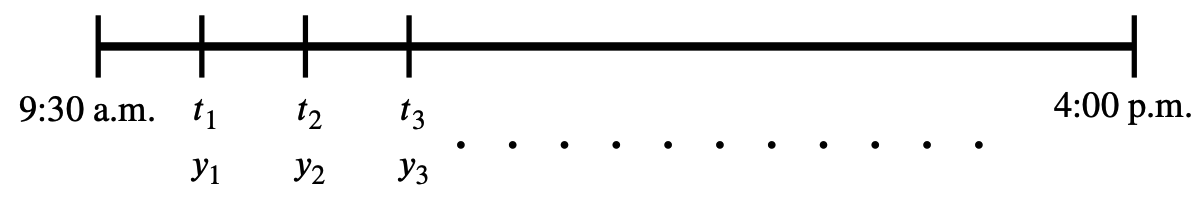
\includegraphics[scale=0.4]{figures/time_series_analysis/ticksandmarks}
\caption{Ticks and Marks}
\end{figure}

A data aggregation method is where aggregation is conducted when there is a change in marker. An alternative aggregation method would be to divide the time span $T$ for exchange hours into $K$ intervals, so regularly spaced intervals are of size $\Delta t = T/K$. The time series method to be discussed will apply to all aggregated data.

Let $p_{it} = \ln P_{it}$ denote price of $i$th asset at time $t$; $p_t = (p_{1t}, p_{2t}, \ldots, p_{nt})$ denote price vector for $n$ assets; $y_{it}$ denote vector of characteristics of $i$th asset at time $t$. These quantities are aggregated from high frequency data. Consider $r$ factors $f_t = (f_{1t}, f_{2t}, \ldots, f_{rt})$ that may include market and industry factors, and asset characteristics. Trading rules can be broadly grouped as follows:
\begin{enumerate}[label=\roman*.]
\setlength{\itemsep}{0pt}
\item \hlt{Statistical Arbitrage}: $E(p_{i, t+1} \ \vert \ p_{i,t}, p_{i, t-1}, \ldots, y_{i,t}, y_{i, t-1}, \ldots)$, that predicts the price of $i$th stock at $t+1$ based on past trading information (also known as time series momentum)
\item \hlt{Momentum}: $E(p_{t+1} \ \vert \ p_t, p_{t-1}, \ldots, y_t, y_{t-1}, \ldots)$, that predicts the cross-sectional momentum of a subset of stocks based on past trading characteristics. For portfolio formation and rebalancing, pairs trading
\item \hlt{Fair Value}: $E(p_{t+1} \ \vert \ p_{t}, p_{t-1}, \ldots, y_t, y_{t-1}, \ldots, f_t, f_{t-1}, \ldots)$, predicts price using all relevant quantities. Factors normally include market, Fama-French; at a more macro level than timescale considered for price prediction, but may still be useful.
\end{enumerate}

Hence price and volatility prediction can be formulated as a time series prediction problem. Autocorrelations and partial autocorrelations can be used to build autoregressive and ARCH models with some predictive power.

Let $Y_1, Y_2, \ldots, Y_T$ be a sequence of random variables with a joint probability distribution. A sequence of observations of stochastic process $\{Y_t, t = 1, \ldots, T\}$ is a realisation of the process.
A time series $\{Y_t\}$ is \hlt{stationary} if for every integer $m$, the set of variables $Y_{t_1}, Y_{t_2}, \ldots, Y_{t_m}$ depends only on the distance between times $t_1, t_2, \ldots, t_m$. Thus $E(Y_t) = \mu$, $Var(Y_t) = \sigma^2$ are constant for all $t$.
The \hlt{auto-covariance} function is defined as
\begin{equation*}
\gamma(s) = Cov(Y_t, Y_{t-s}) = E[(Y_t - \mu)(Y_{t-s} - \mu)] \ \ \forall s = 0, \pm 1, \ldots \nonumber
\end{equation*}
The \hlt{auto-correlation} of process at lag $s$ is defined as
\begin{equation*}
\rho(s) = Corr(Y_t, Y_{t-s}) = \frac{Cov(Y_t, Y_{t-s})}{\left(Var(Y_t) \ Var(Y_{t-s}) \right)^{1/2}} = \frac{\gamma(s)}{\gamma(0)}, \ \ \ \forall s = 0, \pm 1, \ldots \nonumber
\end{equation*}

Some examples of stationary stochastic processes are as follows:

\begin{example} \hlt{(White Noise)} Sequence of discrete independent random variables (r.v.) $\{\epsilon_t \}$ with $E[\epsilon_t] = 0$ and $E[\epsilon_t^2] = \sigma^2$. Set $Y_t = \mu + \epsilon_t$, then $E[Y_t] = \mu$, $Cov(Y_t, Y_{t-s}) = Var(Y_t) = \sigma^2$ if $s=0$, and $Cov(Y_t, Y_{t-s}) = 0$ if $s \neq 0$. Hence the process is stationary.
\end{example}

\begin{example} \hlt{(Moving Average)} Let $\{\epsilon_t\}$ be independent r.v., with process $\{Y_t\}$ where $Y_t = \mu + \epsilon_t + \epsilon_{t_1}$ for $t = 0, 1, 2, \ldots$, and $\mu$ is constant. Then $E[Y_t] = \mu \ \forall t$, and
\begin{equation*}
Cov(Y_t, Y_{t-s}) = \gamma(s) = 
\begin{cases}
2 \sigma^2 \ \ \text{if } s = 0 \\
\sigma^2 \ \ \text{if } s = 1 \\
0 \ \ \text{if } s > 1
\end{cases} \nonumber
\end{equation*}
Hence $\{Y_t\}$ is stationary, with $\rho(s) = \gamma(s) / \gamma(0)$ such that $\rho(0) = 1$, $\rho(1) = 1/2$, $\rho(s) = 0$ for $\abs{s} > 1$.
\end{example}

Some examples of non-stationary stochastic processes are as follows:

\begin{example} \hlt{(Random Walk with Drift)} Let $\{\epsilon_t \}$ be sequence of independent r.v. with  $E[\epsilon_t] = 0$, $E[\epsilon_t^2] = \sigma^2$, and define process $\{Y_t\}$ by $Y_t = Y_{t-1} + \delta + \epsilon_t$ with $Y_0 = 0$. Then the process can be summarised as
\begin{equation*}
Y_t = \delta t + \sum\limits_{j=1}^t \epsilon_j \nonumber
\end{equation*}
Note that $E[Y_t] = \delta t$ and $Var[Y_t] = t \sigma^2$, hence process $\{Y_t\}$ is not stationary.
\end{example}

Given $T$ observations from stationary process $\{Y_t\}$, the \hlt{sample mean} is $\overline{Y} = \frac{1}{T} \sum\limits_{t=1}^T Y_t$. The \hlt{sample auto-covariance} function is defined by $\hat{\gamma}(s) = \frac{1}{T} \sum\limits_{t=1}^{T-s} (Y_t - \overline{Y})(Y_{T-s} - \overline{Y})$ for $s=0, 1, \ldots$. The \hlt{sample auto-correlation} function (ACF) is defined as $\hat{\rho}(s) = \frac{\hat{\gamma}(s)}{\hat{\gamma}(0)} = r(s)$. The \hlt{sample variance} is $Var(\overline{Y}) = \frac{\gamma(0)}{T}\left[1 + 2 \sum\limits_{u=1}^{Y-1} \left(\frac{T-u}{T} \right) \rho(u) \right]$; note that it has to account for auto-correlations.

\begin{definition} A stochastic process $\{Y_t\}$ is a \hlt{linear process} if it can be represented as
\begin{equation*}
Y_t = \mu + \sum\limits_{j=0}^{\infty} \Psi_j \epsilon_{t-j} \nonumber
\end{equation*}
where $\epsilon_t$ are independent with mean $0$, variance $\sigma_{\epsilon}^2$, and $\sum\limits_{j=0}^{\infty} < \infty$.
\end{definition}


\subsection{ARMA and ARIMA Structure}
% AR, MA, ARMA, ARIMA, estimation, forecasting, model diagnostics.

\subsection{Spectral Methods}
% Spectral density, periodogram, filtering, frequency-domain analysis.

\subsection{State-Space Models}
% Linear Gaussian state-space models, Kalman filter, smoothing, prediction.

\subsection{Nonlinear and Volatility Models}
% ARCH/GARCH, stochastic volatility, nonlinear autoregression.

\subsection{Long Memory and Multiscale Structure}
% Fractional processes, long-range dependence, wavelet/time-frequency preview.

\subsection{Sequential Inference and Filtering}
% Hidden Markov models, particle filters, Bayesian filtering, online prediction.

% Sources: Brockwell-Davis, Time Series: Theory and Methods; Hamilton, Time Series Analysis; Durbin-Koopman for state-space methods.
